% Copyright 2009 by Till Tantau
%
% This file may be distributed and/or modified
%
% 1. under the LaTeX Project Public License and/or
% 2. under the GNU Free Documentation License.
%
% See the file doc/generic/pgf/licenses/LICENSE for more details.


% \section{Tutorial: A Picture for Karl's Students}
\section{教程:卡尔学生的图片}

% This tutorial is intended for new users of \tikzname. It does not give an exhaustive account of all the features of \tikzname, just of those that you are likely to use right away. 

本教程适用于\tikzname 的新用户。 它没有详尽介绍\tikzname 的所有功能,只是您可能立即使用的那些功能。

% Karl is a math and chemistry high-school teacher. He used to create the graphics in his worksheets and exams using \LaTeX's |{picture}| environment. While the results were acceptable, creating the graphics often turned out to be a lengthy process. Also, there tended to be problems with lines having slightly wrong angles and circles also seemed to be hard to get right. Naturally, his students could not care less whether the lines had the exact right angles and they find Karl's exams too difficult no matter how nicely they were drawn. But Karl was never entirely satisfied with the result.

卡尔(Karl)是一位数学和化学高中老师。 他曾经使用\LaTeX 的 |{picture}| 环境在练习题和考试中创建图形。 虽然结果是可以接受的,但是创建图形往往是一个漫长的过程。 另外,角度略有错误的直线也容易出现问题,圆也似乎难以正确。 自然,他的学生们并不在乎这些线是否具有正确的直角,并且无论画得多么好,他们都觉得卡尔的考试太难了。 但是卡尔从未对结果完全满意。

% Karl's son, who was even less satisfied with the results (he did not have to take the exams, after all), told Karl that he might wish to try out a new package for creating graphics. A bit confusingly, this package seems to have two names: First, Karl had to download and install a package called \pgfname. Then it turns out that inside this package there is another package called \tikzname, which is supposed to stand for ``\tikzname\ ist \emph{kein} Zeichenprogramm''. Karl finds this all a bit strange and \tikzname\ seems to indicate that the package does not do what he needs. However, having used \textsc{gnu} software for quite some time and ``\textsc{gnu} not being Unix'', there seems to be hope yet. His son assures him that \tikzname's name is intended to warn people that \tikzname\ is not a program that you can use to draw graphics with your mouse or tablet. Rather, it is more like a ``graphics language''. 

卡尔的儿子对这样的结果并不满意(毕竟他不必参加考试),他告诉卡尔,他可能希望尝试一种用于制作图形的新的宏包。 有点令人困惑的是,该宏包似乎有两个名称:首先,卡尔必须下载并安装一个名为\pgfname 的宏包。 然后事实证明,在该程序包中还有另一个名为\tikzname 的宏包,它应该表示``\tikzname\ ist \emph{kein} Zeichenprogramm(\tikzname 不是一个绘图程序)''。  卡尔发现这一切都有些奇怪,\tikzname\ 似乎表明该宏包无法满足他的需要。 但是,使用\textsc{gnu}软件已经有一段时间了,并且``\textsc{gnu}不是Unix'',似乎还有希望。 他的儿子向他保证,\tikzname\ 的名称旨在警告人们,\tikzname\ 不是可用于使用鼠标或平板电脑绘制图形的程序。 相反,它更像是一种``图形语言''。

% \subsection{Problem Statement}
\subsection{问题描述}

% Karl wants to put a graphic on the next worksheet for his students. He is currently teaching his students about sine and cosine. What he would like to have is something that looks like this (ideally):

卡尔希望在下一次练习题中为他的学生添加一张图解。 他目前正在向学生教授正弦和余弦。 他想绘制的图形(理想情况下)如下所示:

%
\noindent
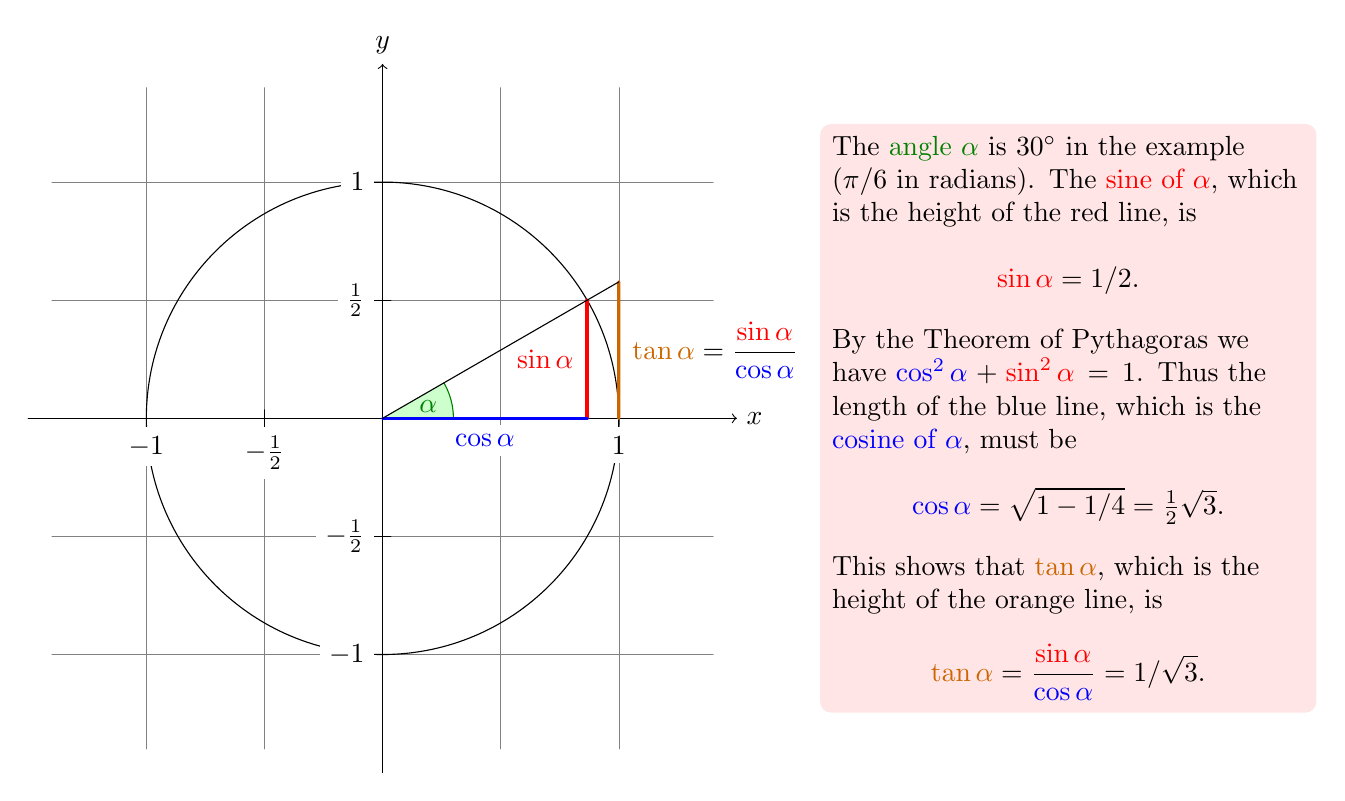
\begin{tikzpicture}
  [scale=3,line cap=round,
   % Styles
   axes/.style=,
   important line/.style={very thick},
   information text/.style={rounded corners,fill=red!10,inner sep=1ex}]

  % Local definitions
  \def\costhirty{0.8660256}

  % Colors
  \colorlet{anglecolor}{green!50!black}
  \colorlet{sincolor}{red}
  \colorlet{tancolor}{orange!80!black}
  \colorlet{coscolor}{blue}

  % The graphic
  \draw[help lines,step=0.5cm] (-1.4,-1.4) grid (1.4,1.4);

  \draw (0,0) circle [radius=1cm];

  \begin{scope}[axes]
    \draw[->] (-1.5,0) -- (1.5,0) node[right] {$x$};
    \draw[->] (0,-1.5) -- (0,1.5) node[above] {$y$};

    \foreach \x/\xtext in {-1, -.5/-\frac{1}{2}, 1}
      \draw[xshift=\x cm] (0pt,1pt) -- (0pt,-1pt) node[below,fill=white] {$\xtext$};

    \foreach \y/\ytext in {-1, -.5/-\frac{1}{2}, .5/\frac{1}{2}, 1}
      \draw[yshift=\y cm] (1pt,0pt) -- (-1pt,0pt) node[left,fill=white] {$\ytext$};
  \end{scope}

  \filldraw[fill=green!20,draw=anglecolor] (0,0) -- (3mm,0pt) arc(0:30:3mm);
  \draw (15:2mm) node[anglecolor] {$\alpha$};

  \draw[important line,sincolor]
    (30:1cm) -- node[left=1pt,fill=white] {$\sin \alpha$} +(0,-.5);

  \draw[important line,coscolor]
    (0,0) -- node[below=2pt,fill=white] {$\cos \alpha$} (\costhirty,0);

  \draw[important line,tancolor] (1,0) --
    node [right=1pt,fill=white]
    {
      $\displaystyle \tan \alpha \color{black}=
      \frac{{\color{sincolor}\sin \alpha}}{\color{coscolor}\cos \alpha}$
    } (intersection of 0,0--30:1cm and 1,0--1,1) coordinate (t);

  \draw (0,0) -- (t);

  \draw[xshift=1.85cm] node [right,text width=6cm,information text]
    {
      The {\color{anglecolor} angle $\alpha$} is $30^\circ$ in the example ($\pi/6$ in radians). The {\color{sincolor}sine of $\alpha$}, which is the height of the red line, is

      % 示例中,{\color{anglecolor}角度$\alpha$}为$30^\circ$(弧度为$\pi/6$)。 {$\alpha$的\color{sincolor}正弦值},即红线的高度,为
      \[
      {\color{sincolor} \sin \alpha} = 1/2.
      \]

      By the Theorem of Pythagoras we have ${\color{coscolor}\cos^2 \alpha} + {\color{sincolor}\sin^2\alpha} =1$. Thus the length of the blue line, which is the {\color{coscolor}cosine of $\alpha$}, must be

      % 根据勾股定理,我们得到${\color{coscolor}\cos^2 \alpha} + {\color{sincolor}\sin^2\alpha} =1$。 因此,蓝线的长度应该是{\color{coscolor} $\alpha$}的余弦
      \[
      {\color{coscolor}\cos\alpha} = \sqrt{1 - 1/4} = \textstyle
      \frac{1}{2} \sqrt 3.
      \]%
      This shows that {\color{tancolor}$\tan \alpha$}, which is the height of the orange line, is
      
      % 这表明{\color{tancolor} $\tan\alpha$},即橙线的高度,为
      \[
      {\color{tancolor}\tan\alpha} = \frac{{\color{sincolor}\sin
          \alpha}}{\color{coscolor}\cos \alpha} = 1/\sqrt 3.
      \]%
    };
\end{tikzpicture}

% \subsection{Setting up the Environment}
\subsection{配置环境}

% In \tikzname, to draw a picture, at the start of the picture you need to tell \TeX\ or \LaTeX\ that you want to start a picture. In \LaTeX\ this is done using the environment |{tikzpicture}|, in plain \TeX\ you just use |\tikzpicture| to start the picture and |\endtikzpicture| to end it. 

在\tikzname 中绘制图片,在图片的开头,您需要告诉\TeX\ 或\LaTeX\ 您要开始绘制图片。在\LaTeX\ 中,这是使用 |{tikzpicture}| 环境完成的,在Plain \TeX\ 中,您只需使用 |\tikzpicture| 开始绘制图片以及使用 |\endtikzpicture| 结束绘制。

% \subsubsection{Setting up the Environment in \LaTeX}
\subsubsection{在\LaTeX 中配置环境}

% Karl, being a \LaTeX\ user, thus sets up his file as follows:

卡尔作为一个\LaTeX\ 用户,他的文件如下:

%
\begin{codeexample}[code only]
\documentclass{article} % say
\usepackage{tikz}
\begin{document}
We are working on
\begin{tikzpicture}
  \draw (-1.5,0) -- (1.5,0);
  \draw (0,-1.5) -- (0,1.5);
\end{tikzpicture}.
\end{document}
\end{codeexample}

% When executed, that is, run via |pdflatex| or via |latex| followed by |dvips|, the resulting will contain something that looks like this:

执行后,即通过运行 |pdflatex| 或通过运行 |latex| 然后运行 |dvips|,结果将包含如下内容:

%
\begin{codeexample}[width=7cm]
We are working on
\begin{tikzpicture}
  \draw (-1.5,0) -- (1.5,0);
  \draw (0,-1.5) -- (0,1.5);
\end{tikzpicture}.
\end{codeexample}

% Admittedly, not quite the whole picture, yet, but we do have the axes established. Well, not quite, but we have the lines that make up the axes drawn. Karl suddenly has a sinking feeling that the picture is still some way off.

诚然,这还不是全部,但我们确实已经确定了坐标轴。 好吧,虽然不完全,但是我们有构成绘制坐标轴的线。 卡尔突然感到那张图解还差得远。

% Let's have a more detailed look at the code. First, the package |tikz| is loaded. This package is a so-called ``frontend'' to the basic \pgfname\ system. The basic layer, which is also described in this manual, is somewhat more, well, basic and thus harder to use. The frontend makes things easier by providing a simpler syntax. 

让我们更详细地看一下代码。 首先,包 |tikz| 已加载。该软件包是基本\pgfname\ 系统的所谓的``前端''。本手册中也介绍了基础层,它更基础一些,因此也更难使用。前端通过提供更简单的语法使事情变得更容易。

% Inside the environment there are two |\draw| commands. They mean: ``The path, which is specified following the command up to the semicolon, should be drawn.'' The first path is specified as |(-1.5,0) -- (0,1.5)|, which means ``a straight line from the point at position $(-1.5,0)$ to the point at position $(0,1.5)$''. Here, the positions are specified within a special coordinate system in which, initially, one unit is 1cm.

在环境内部有两个 |\draw| 命令。它们的意思是:“应该绘制从命令到分号为止指定的路径。”第一个路径指定为 |(-1.5,0) -- (0,1.5)|,表示`“从位置$(-1.5,0)$到位置$(0,1.5)$的直线”。在此,位置是在特殊坐标系中指定的,初始条件下,一个单位为1厘米。

% Karl is quite pleased to note that the environment automatically reserves enough space to encompass the picture. 

卡尔非常高兴地注意到环境会自动保留足够的空间来容纳图片。

% \subsubsection{Setting up the Environment in Plain \TeX}
\subsubsection{在Plain \TeX 中配置环境}

% Karl's wife Gerda, who also happens to be a math teacher, is not a \LaTeX\ user, but uses plain \TeX\ since she prefers to do things ``the old way''. She can also use \tikzname. Instead of |\usepackage{tikz}| she has to write |\input tikz.tex| and instead of |\begin{tikzpicture}| she writes |\tikzpicture| and instead of |\end{tikzpicture}| she writes |\endtikzpicture|.

卡尔的妻子格达(Gerda)恰好也是一名数学老师,她不是\LaTeX\ 用户,而使用Plain \TeX\ ,因为她更喜欢以``旧方式''做事。她还可以使用\tikzname 。她必须使用 |\inputtikz.tex| 代替 |\usepackage{tikz}|,使用 |\tikzpicture| 代替 |\begin{tikzpicture}| 以及使用 |\endtikzpicture| 代替 |\end{tikzpicture}|。

% Thus, she would use:

因此,她将使用:

%
\begin{codeexample}[code only]
%% Plain TeX file
\input tikz.tex
\baselineskip=12pt
\hsize=6.3truein
\vsize=8.7truein
We are working on
\tikzpicture
  \draw (-1.5,0) -- (1.5,0);
  \draw (0,-1.5) -- (0,1.5);
\endtikzpicture.
\bye
\end{codeexample}

% Gerda can typeset this file using either |pdftex| or |tex| together with |dvips|. \tikzname\ will automatically discern which driver she is using. If she wishes to use |dvipdfm| together with |tex|, she either needs to modify the file |pgf.cfg| or can write |\def\pgfsysdriver{pgfsys-dvipdfm.def}| somewhere \emph{before} she inputs |tikz.tex| or |pgf.tex|.

格达可以使用 |pdftex| 或者 |tex| 和 |dvips| 来排版这个文件。\tikzname\ 将自动识别她正在使用哪个驱动程序。如果她希望同时使用 |dvipdfm| 和 |tex|,那么她需要修改文件 |pgf.cfg| 或可以在她输入 |tikz.tex| 或 |pgf.tex| 的位置\emph{之前}添加 |\def\pgfsysdriver{pgfsys-dvipdfm.def}|。


% \subsubsection{Setting up the Environment in Con\TeX t}
\subsubsection{在 Con\TeX t 中配置环境}

% Karl's uncle Hans uses Con\TeX t. Like Gerda, Hans can also use \tikzname. Instead of |\usepackage{tikz}| he says |\usemodule[tikz]|. Instead of |\begin{tikzpicture}| he writes |\starttikzpicture| and  instead of |\end{tikzpicture}| he writes |\stoptikzpicture|.

卡尔的叔叔汉森(Hans)使用Con\TeX t。与格达一样,汉森也可以使用\tikzname 。他将使用 |\usemodule[tikz]| 代替 |\usepackage{tikz}|。使用 |\starttikzpicture| 代替 |\begin{tikzpicture}|,使用 |\stoptikzpicture| 代替 |\end{tikzpicture}|。

% His version of the example looks like this:

他的示例版本如下所示:

%
\begin{codeexample}[code only]
%% ConTeXt file
\usemodule[tikz]

\starttext
  We are working on
  \starttikzpicture
    \draw (-1.5,0) -- (1.5,0);
    \draw (0,-1.5) -- (0,1.5);
  \stoptikzpicture.
\stoptext
\end{codeexample}

% Hans will now typeset this file in the usual way using |texexec| or |context|.

汉森现在将使用 |texexec| 或 |context|,并且以通常的方式排版此文件。


% \subsection{Straight Path Construction}
\subsection{直线路径的创建}

% The basic building block of all pictures in \tikzname\ is the path. A \emph{path} is a series of straight lines and curves that are connected (that is not the whole picture, but let us ignore the complications for the moment). You start a path by specifying the coordinates of the start position as a point in round brackets, as in |(0,0)|. This is followed by a series of ``path extension operations''. The simplest is |--|, which we used already. It must be followed by another coordinate and it extends the path in a straight line to this new position. For example, if we were to turn the two paths of the axes into one path, the following would result:

\tikzname\ 中所有图片的基本构造块是路径。一个\emph{路径}是一系列相连的直线和曲线(这不是全部,但让我们暂时忽略复杂性)。通过将起始位置的坐标指定为方括号中的点来启动路径,如 |(0,0)| 中所示。接下来是一系列“路径扩展操作”。最简单的是 |--|,我们已经用过了。它必须跟随着另一个坐标,它将路径以直线延伸到这个新位置。例如,如果我们将坐标轴的两条路径变换为一条路径,会得到如下结果:

%
\begin{codeexample}[]
\tikz \draw (-1.5,0) -- (1.5,0) -- (0,-1.5) -- (0,1.5);
\end{codeexample}

% Karl is a bit confused by the fact that there is no |{tikzpicture}| environment, here. Instead, the little command |\tikz| is used. This command either takes one argument (starting with an opening brace as in |\tikz{\draw (0,0) -- (1.5,0)}|, which yields \tikz{\draw (0,0) --(1.5,0);}) or collects everything up to the next semicolon and puts it inside a |{tikzpicture}| environment. As a rule of thumb, all \tikzname\ graphic drawing commands must occur as an argument of |\tikz| or inside a |{tikzpicture}| environment. Fortunately, the command |\draw| will only be defined inside this environment, so there is little chance that you will accidentally do something wrong here.

卡尔对这里没有 |{tikzpicture}| 环境这一事实感到有点困惑。相反,使用小命令 | \tikz|。这个命令要么接受一个参数(以 |\tikz{\draw(0,0)--(1.5,0)}| 中的括号开始,这会产生\tikz{\draw(0,0)--(1.5,0);}),要么收集所有内容,直到下一个分号,并将其放到 |{tikzpicture}| 环境中。根据经验,所有\tikzname\ 图形绘制命令都必须作为 |\tikz| 的参数出现,或者出现在 |{tikzpicture}| 环境中。幸运的是,命令 |\draw| 将只在这个环境中定义,因此您不太可能在这里意外地出错。


% \subsection{Curved Path Construction}
\subsection{曲线路径的创建}

% The next thing Karl wants to do is to draw the circle. For this, straight lines obviously will not do. Instead, we need some way to draw curves. For this, \tikzname\ provides a special syntax. One or two ``control points'' are needed. The math behind them is not quite trivial, but here is the basic idea: Suppose you are at point $x$ and the first control point is $y$. Then the curve will start ``going in the direction of~$y$ at~$x$'', that is, the tangent of the curve at $x$ will point toward~$y$. Next, suppose the curve should end at $z$ and the second support point is $w$. Then the curve will, indeed, end at $z$ and the tangent of the curve at point $z$ will go through $w$.

卡尔想做的下一件事是画圆。对于这个问题,直线显然是不行的。相反,我们需要一些绘制曲线的方法。为此,\tikzname\ 提供了特殊的语法。需要一两个“控制点”。它们背后的数学原理并不简单,但基本的思想是:假设您在点$x$,第一个控制点是$y$。然后曲线将开始朝着~$y$在~$x$的方向,也就是说,曲线在$x$处的切线将指向~$y$。接下来,假设曲线应该结束于$z$,第二个控制点是$w$。曲线会在$z$点结束曲线在$z$点的切线会经过$w$点。

% Here is an example (the control points have been added for clarity):

这是一个示例(为清楚起见添加了控制点):

%
\begin{codeexample}[]
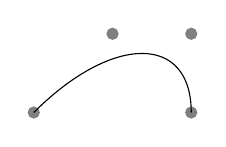
\begin{tikzpicture}
  \filldraw [gray] (0,0) circle [radius=2pt]
                   (1,1) circle [radius=2pt]
                   (2,1) circle [radius=2pt]
                   (2,0) circle [radius=2pt];
  \draw (0,0) .. controls (1,1) and (2,1) .. (2,0);
\end{tikzpicture}
\end{codeexample}

% The general syntax for extending a path in a ``curved'' way is |.. controls| \meta{first control point} |and| \meta{second control point} |..| \meta{end point}. You can leave out the |and| \meta{second control point}, which causes the first one to be used twice.

% 以“弯曲”方式扩展路径的一般语法是| ..控件|  \ meta {第一个控制点} |和|  \ meta {第二控制点} | .. |  \ meta {end point}。 您可以忽略|和|  \ meta {第二控制点},这会使第一个控制点使用两次。

以“弯曲”方式扩展路径的一般语法是 |.. controls| \meta{第一个控制点} |and| \meta{第二个控制点} |..|。您可以省略 |and| \meta{第二个控制点},这将使第一个控制点被使用两次。

% So, Karl can now add the first half circle to the picture:

因此,卡尔现在可以将前半圆添加到图片中:

%
\begin{codeexample}[]
\begin{tikzpicture}
  \draw (-1.5,0) -- (1.5,0);
  \draw (0,-1.5) -- (0,1.5);
  \draw (-1,0) .. controls (-1,0.555) and (-0.555,1) .. (0,1)
               .. controls (0.555,1) and (1,0.555) .. (1,0);
\end{tikzpicture}
\end{codeexample}

% Karl is happy with the result, but finds specifying circles in this way to be extremely awkward. Fortunately, there is a much simpler way.

卡尔对结果感到满意,但是发现以这种方式指定圆非常尴尬。 幸运的是,有一种更简单的方法。


% \subsection{Circle Path Construction}
\subsection{圆路径的创建}

% In order to draw a circle, the path construction operation |circle| can be used. This operation is followed by a radius in brackets as in the following example: (Note that the previous position is used as the \emph{center} of the circle.)

为了画一个圆,可以使用路径构建运算符 |circ|。 此运算符后跟方括号中的半径,如以下示例所示:(请注意,运算符之前的位置用作圆的\emph{圆心}。)

%
\begin{codeexample}[]
\tikz \draw (0,0) circle [radius=10pt];
\end{codeexample}

% You can also append an ellipse to the path using the |ellipse| operation. Instead of a single radius you can specify two of them:

您也可以使用 |ellipse| 操作添加椭圆路径。 您可以指定两个,而不是单个半径:

%
\begin{codeexample}[]
\tikz \draw (0,0) ellipse [x radius=20pt, y radius=10pt];
\end{codeexample}

% To draw an ellipse whose axes are not horizontal and vertical, but point in an arbitrary direction (a ``turned ellipse'' like \tikz \draw[rotate=30] (0,0) ellipse [x radius=6pt, y radius=3pt];) you can use transformations, which are explained later. The code for the little ellipse is |\tikz \draw[rotate=30] (0,0) ellipse [x radius=6pt, y radius=3pt];|, by the way.

要绘制的轴线不是水平和竖直的,而是指向任意方向的椭圆(一个像这样旋转后的椭圆\tikz \draw[rotate=30] (0,0) ellipse [x radius=6pt, y radius=3pt];),您可以使用旋转,稍后将对此进行解释。顺便提一下,小椭圆的代码是 |\tikz \draw[rotate=30] (0,0) ellipse [x radius=6pt, y radius=3pt];|。

% So, returning to Karl's problem, he can write |\draw (0,0) circle [radius=1cm];| to draw the circle:

那么,回到卡尔的问题,他可以写 |\draw (0,0) circle [radius=1cm];| 画圆:

%
\begin{codeexample}[]
\begin{tikzpicture}
  \draw (-1.5,0) -- (1.5,0);
  \draw (0,-1.5) -- (0,1.5);
  \draw (0,0) circle [radius=1cm];
\end{tikzpicture}
\end{codeexample}

% At this point, Karl is a bit alarmed that the circle is so small when he wants the final picture to be much bigger. He is pleased to learn that \tikzname\ has powerful transformation options and scaling everything by a factor of three is very easy. But let us leave the size as it is for the moment to save some space.

在这一点上,卡尔有点惊慌,圆是如此之小,他想要最后的图片大得多。他很高兴地了解到\tikzname\ 具有强大的变换选项,并且很容易将所有内容放大到原来的三倍。但是为了节省一些空间,让我们暂时保持大小不变。


% \subsection{Rectangle Path Construction}
\subsection{矩形路径的创建}

% The next things we would like to have is the grid in the background. There are several ways to produce it. For example, one might draw lots of rectangles. Since rectangles are so common, there is a special syntax for them: To add a rectangle to the current path, use the |rectangle| path construction operation. This operation should be followed by another coordinate and will append a rectangle to the path such that the previous coordinate and the next coordinates are corners of the rectangle. So, let us add two rectangles to the picture:

接下来我们想要的是背景中的网格。有几种方法可以产生它。例如,有人可能会画很多矩形。由于矩形非常常见,因此它们有一种特殊的语法:要向当前路径添加矩形,我们使用 |rectangle| 路径构造操作。该操作之后应该跟着另一个坐标,并将一个矩形添加到路径中,使前一个坐标和下一个坐标都是矩形的角点。所以,我们添加两个矩形的图片:

%
\begin{codeexample}[]
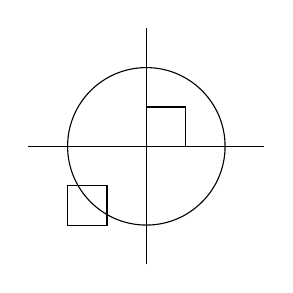
\begin{tikzpicture}
  \draw (-1.5,0) -- (1.5,0);
  \draw (0,-1.5) -- (0,1.5);
  \draw (0,0) circle [radius=1cm];
  \draw (0,0) rectangle (0.5,0.5);
  \draw (-0.5,-0.5) rectangle (-1,-1);
\end{tikzpicture}
\end{codeexample}

% While this may be nice in other situations, this is not really leading anywhere with Karl's problem: First, we would need an awful lot of these rectangles and then there is the border that is not ``closed''.

虽然这在其他情况下可能很好,但这并没有真正解决卡尔的问题:首先,我们需要大量的矩形,然后边界没有“封闭”。

% So, Karl is about to resort to simply drawing four vertical and four horizontal lines using the nice |\draw| command, when he learns that there is a |grid| path construction operation. 

因此,当卡尔得知有一个 |grid| 路径构造操作时,他打算使用漂亮的 |\draw| 命令简单地绘制四条垂直和四条水平线。

% \subsection{Grid Path Construction}
\subsection{网格路径的创建}

% The |grid| path operation adds a grid to the current path. It will add lines making up a grid that fills the rectangle whose one corner is the current point and whose other corner is the point following the |grid| operation. For example, the code |\tikz \draw[step=2pt] (0,0) grid (10pt,10pt);| produces \tikz \draw[step=2pt] (0,0) grid (10pt,10pt);. Note how the optional argument for |\draw| can be used to specify a grid width (there are also |xstep| and |ystep| to define the steppings independently). As Karl will learn soon, there are \emph{lots} of things that can be influenced using such options.

|grid| 路径操作向当前路径添加一个网格。它将添加组成网格的线,填充矩形,矩形的一个角点是当前点,另一个角点是紧跟 |grid| 操作的点。例如,代码 |\tikz \draw[step=2pt] (0,0) grid (10pt,10pt);| 生成 \tikz \draw[step=2pt] (0,0) grid (10pt,10pt);。请注意,可以使用 |\draw| 的可选参数来指定网格宽度(还有 |xstep| 和 |ystep| 来分别定义步长)。卡尔很快就会了解到,使用这些选项可以影响到\emph{很多}事情。

% For Karl, the following code could be used:

对于卡尔来说,可以使用以下代码:

%
\begin{codeexample}[]
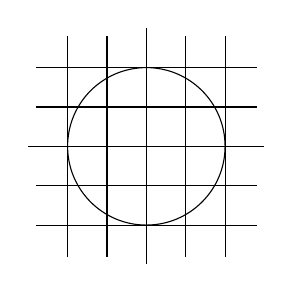
\begin{tikzpicture}
  \draw (-1.5,0) -- (1.5,0);
  \draw (0,-1.5) -- (0,1.5);
  \draw (0,0) circle [radius=1cm];
  \draw[step=.5cm] (-1.4,-1.4) grid (1.4,1.4);
\end{tikzpicture}
\end{codeexample}

% Having another look at the desired picture, Karl notices that it would be nice for the grid to be more subdued. (His son told him that grids tend to be distracting if they are not subdued.) To subdue the grid, Karl adds two more options to the |\draw| command that draws the grid. First, he uses the color |gray| for the grid lines. Second, he reduces the line width to |very thin|. Finally, he swaps the ordering of the commands so that the grid is drawn first and everything else on top.

再次查看所需的图片后,卡尔注意到,使网格的颜色更浅一点会很好。(他的儿子告诉他,如果不使网格的颜色变浅,网格往往会分散注意力。)为了使网格的颜色变浅,卡尔在 |\draw| 命令中添加了两个选项。首先,他使用 |gray| 颜色表示网格线。 其次,他将线宽减小到 |very thin|。 最后,他交换命令的顺序,以便首先绘制网格,然后再绘制其他所有内容。

%
\begin{codeexample}[]
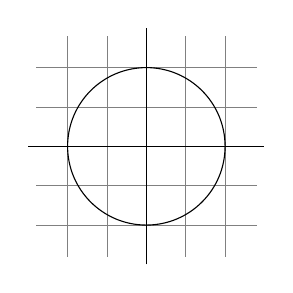
\begin{tikzpicture}
  \draw[step=.5cm,gray,very thin] (-1.4,-1.4) grid (1.4,1.4);
  \draw (-1.5,0) -- (1.5,0);
  \draw (0,-1.5) -- (0,1.5);
  \draw (0,0) circle [radius=1cm];
\end{tikzpicture}
\end{codeexample}


% \subsection{Adding a Touch of  Style}
\subsection{增加一点风格}

% Instead of the options |gray,very thin| Karl could also have said |help lines|. \emph{Styles} are predefined sets of options that can be used to organize how a graphic is drawn. By saying |help lines| you say ``use the style that I (or someone else) has set for drawing help lines''. If Karl decides, at some later point, that grids should be drawn, say, using the color |blue!50| instead of |gray|, he could provide the following option somewhere:

除了使用选项 |gray,very thin|,卡尔也可以声明 |help lines|。 \emph{Styles}是预定义的选项集,可用于组织图形的绘制方式。 通过声明 |help lines| 相当于您说“使用我(或其他人)设置的样式来绘制辅助线”。 如果卡尔在以后的某个时刻决定应该绘制网格,例如使用 |blue!50| 颜色代替 |gray|,他可以在某处提供以下选项:

%
\begin{codeexample}[code only]
help lines/.style={color=blue!50,very thin}
\end{codeexample}
%
%The effect of this ``style setter'' is that in the current scope or environment the |help lines| option has the same effect as |color=blue!50,very thin|.

这种``样式设置器''的作用是,在当前分组或环境中 |help lines| 选项与 |color=blue!50,very thin| 的效果相同。

% Using styles makes your graphics code more flexible. You can change the way things look easily in a consistent manner. Normally, styles are defined at the beginning of a picture. However, you may sometimes wish to define a style globally, so that all pictures of your document can use this style. Then you can easily change the way all graphics look by changing this one style. In this situation you can use the |\tikzset| command at the beginning of the document as in

使用样式可使您的图形代码更加灵活。 您可以以一致的方式更改事物看起来的方式。 通常,样式是在图片的开头定义的。 但是,有时您可能希望全局定义样式,以便文档的所有图片都可以使用此样式。 然后,您可以通过更改一种样式轻松更改所有图形的外观。 在这种情况下,您可以在文档开头使用 |\tikzset| 命令,如

%
\begin{codeexample}[code only]
\tikzset{help lines/.style=very thin}
\end{codeexample}

% To build a hierarchy of styles you can have one style use another. So in order to define a style |Karl's grid| that is based on the |grid| style Karl could say

要建立样式的层级结构,您可以让一种样式使用另一种样式。 因此,为了定义基于 |grid| 风格的样式 |Karl's grid| 卡尔可以这样声明

%
\begin{codeexample}[code only]
\tikzset{Karl's grid/.style={help lines,color=blue!50}}
...
\draw[Karl's grid] (0,0) grid (5,5);
\end{codeexample}

% Styles are made even more powerful by parametrization. This means that, like other options, styles can also be used with a parameter. For instance, Karl could parameterize his grid so that, by default, it is blue, but he could also use another color.

通过参数化,样式变得更加强大。 这意味着,与其他选项一样,样式也可以与参数一起使用。 例如,卡尔可以对网格进行参数化,以便默认情况下为蓝色,但是他也可以使用其他颜色。

%
\begin{codeexample}[code only]
\begin{tikzpicture}
  [Karl's grid/.style  ={help lines,color=#1!50},
   Karl's grid/.default=blue]

  \draw[Karl's grid]     (0,0) grid (1.5,2);
  \draw[Karl's grid=red] (2,0) grid (3.5,2);
\end{tikzpicture}
\end{codeexample}

% In this example, the definition of the style |Karl's grid| is given as an  optional argument to the |{tikzpicture}| environment. Additional styles for other  elements would follow after a comma. With many styles in effect, the optional  argument of the environment may easily happen to be longer than the actual contents.

在此示例中,样式 |Karl's grid| 的定义用作 |{tikzpicture}| 环境的可选参数。 其他元素的附加样式将紧跟在逗号之后。 在使用多种样式的情况下,环境的可选参数可能很容易长于实际内容。

% \subsection{Drawing Options}
\subsection{绘图选项}

% Karl wonders what other options there are that influence how a path is drawn. He saw already that the |color=|\meta{color} option can be used to set the line's color. The option |draw=|\meta{color} does nearly the same, only it sets the color for the lines only and a different color can be used for filling (Karl will need this when he fills the arc for the angle). 

卡尔想知道还有什么其他选项可以影响路径的绘制。他已经看到可以使用 |color=| \meta{color} 选项来设置线条的颜色。选项 |draw=| \meta{color} 做的几乎是一样的,只是它只设置了线条的颜色,可以使用不同的颜色填充(卡尔填充圆弧的角度会用到这个选项)。

% He saw that the style |very thin| yields very thin lines. Karl is not really surprised by this and neither is he surprised to learn that |thin| yields thin lines,  |thick| yields thick lines, |very thick| yields very thick lines, |ultra thick| yields really, really thick lines and |ultra thin| yields lines that are so thin that low-resolution printers and displays will have trouble showing them. He wonders what gives lines of ``normal'' thickness. It turns out that |thin| is the correct choice, since it gives the same thickness as \TeX's |\hrule| command. Nevertheless, Karl would like to know whether there is anything ``in the middle'' between |thin| and |thick|. There is: |semithick|.

他看到样式 |very thin| 产生非常细的线。 卡尔对此并不感到惊讶,也不会惊讶于 |thin| 产生细线,|thick| 产生的粗线,|very thick| 产生非常粗的线,|ultra thick| 产生非常非常粗的线以及 |ultra thin| 产生非常非常细的线,以至于低分辨率的打印机和显示器将很难显示它们。 他想知道是什么使线条具有``正常''的宽度。 事实证明 |thin| 是正确的选择,因为它的厚度与\TeX 的 |\hrule| 命令相同。 但是,卡尔想知道 |thin| 和 |thick| 之间是否有“中间”的宽度。有:|semithick|。

% Another useful thing one can do with lines is to dash or dot them. For this, the two styles |dashed| and |dotted| can be used, yielding \tikz[baseline] \draw[dashed] (0,.5ex) -- ++(2em,0pt); and \tikz[baseline] \draw[dotted] (0,.5ex) -- ++(2em,0pt);. Both options also exist in a loose and a dense version, called |loosely dashed|, |densely dashed|, |loosely dotted|, and |densely dotted|. If he really, really  needs to, Karl can also define much more complex dashing patterns with the |dash pattern| option, but his son insists that dashing is to be used with utmost care and mostly distracts. Karl's son claims that complicated dashing patterns are evil. Karl's students do not care about dashing patterns.

对线条的另一种有用的处理是虚线或点线。为此,可以使用 |dashed| 和 |dotted| 两种样式,产生\tikz[baseline] \draw[dashed] (0,.5ex) -- ++(2em,0pt);和\tikz[baseline] \draw[dotted] (0,.5ex) -- ++(2em,0pt);。这两个选项也存在松散和密集的版本,称为 |loosely dashed|,|densely dashed|,|loosely dotted|,|densely dotted|。如果他真的真的需要,卡尔也可以使用 |dash pattern| 选项定义更复杂的虚线样式,但他的儿子坚持认为,在使用时要格外小心,而且大多会分散注意力。卡尔的儿子声称复杂的虚线图案是邪恶的。卡尔的学生不关心虚线的样式。


% \subsection{Arc Path Construction}
\subsection{弧线路径的创建}

% Our next obstacle is to draw the arc for the angle. For this, the |arc| path construction operation is useful, which draws part of a circle or ellipse. This |arc| operation is followed by options in brackets that specify the arc. An example would be |arc[start angle=10, end angle=80, radius=10pt]|, which means exactly what it says. Karl obviously needs an arc from $0^\circ$ to $30^\circ$. The radius should be something relatively small, perhaps around one third of the circle's radius. When one uses the arc path construction operation, the specified arc will be added with its starting point at the current position. So, we first have to ``get there''.

我们的下一个障碍是绘制该角度的弧线。 为此,|arc| 路径构造操作非常有用,它可以绘制一部分圆或椭圆。 |arc| 操作之后的括号指定圆弧的选项。 一个示例是 |arc [start angle=10, end angle=80, radius=10pt]|,其含义就像它说的那样。 卡尔显然需要从$0^\circ$到$30^\circ$的弧线。 半径应相对较小,可能约为圆半径的三分之一。 当使用弧形路径构造操作时,指定的弧形将以其起始点添加到当前位置。 因此,我们首先必须``到达那里''。

%
\begin{codeexample}[]
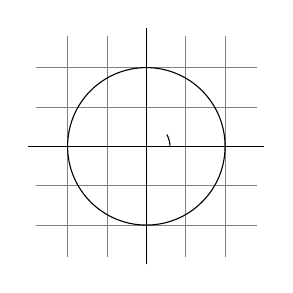
\begin{tikzpicture}
  \draw[step=.5cm,gray,very thin] (-1.4,-1.4) grid (1.4,1.4);
  \draw (-1.5,0) -- (1.5,0);
  \draw (0,-1.5) -- (0,1.5);
  \draw (0,0) circle [radius=1cm];
  \draw (3mm,0mm) arc [start angle=0, end angle=30, radius=3mm];
\end{tikzpicture}
\end{codeexample}

% Karl thinks this is really a bit small and he cannot continue unless he learns how to do scaling. For this, he can add the |[scale=3]| option. He could add this option to each |\draw| command, but that would be awkward. Instead, he adds it to the whole environment, which causes this option to apply to everything within.

卡尔认为这确实有点小,除非学会了缩放方法,否则他无法继续。 为此,他可以添加 \verb|[scale=3]| 选项。 他可以将此选项添加到每个 |\draw| 命令中,但那样做非常麻烦。相反,他将其添加到整个环境中,这使得该选项应用于其中的所有内容。

%
\begin{codeexample}[]
\begin{tikzpicture}[scale=3]
  \draw[step=.5cm,gray,very thin] (-1.4,-1.4) grid (1.4,1.4);
  \draw (-1.5,0) -- (1.5,0);
  \draw (0,-1.5) -- (0,1.5);
  \draw (0,0) circle [radius=1cm];
  \draw (3mm,0mm) arc [start angle=0, end angle=30, radius=3mm];
\end{tikzpicture}
\end{codeexample}

% As for circles, you can specify ``two'' radii in order to get an elliptical arc.

对于圆而言,您可以指定``两个''半径以获得椭圆弧。

%
\begin{codeexample}[]
  \tikz \draw (0,0)
    arc [start angle=0, end angle=315,
         x radius=1.75cm, y radius=1cm];
\end{codeexample}


% \subsection{Clipping a Path}
\subsection{剪切路径}

% In order to save space in this manual, it would be nice to clip Karl's graphics a bit so that we can focus on the ``interesting'' parts. Clipping is pretty easy in \tikzname. You can use the |\clip| command to clip all subsequent drawing. It works like |\draw|, only it does not draw anything, but uses the given path to clip everything subsequently.

为了节省空间,最好裁剪一下卡尔的图形,以便我们专注于“有趣的”部分。 \tikzname 中的剪切非常容易。 您可以使用 |\clip| 命令剪切所有后续图形。 它的工作方式类似于 |\draw|,只是它不绘制任何内容,而是使用给定的路径剪切所有的图形。

%
\begin{codeexample}[]
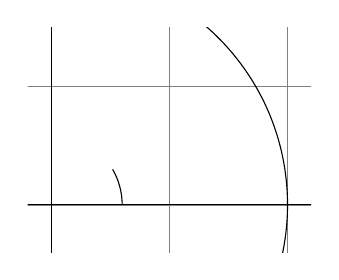
\begin{tikzpicture}[scale=3]
  \clip (-0.1,-0.2) rectangle (1.1,0.75);
  \draw[step=.5cm,gray,very thin] (-1.4,-1.4) grid (1.4,1.4);
  \draw (-1.5,0) -- (1.5,0);
  \draw (0,-1.5) -- (0,1.5);
  \draw (0,0) circle [radius=1cm];
  \draw (3mm,0mm) arc [start angle=0, end angle=30, radius=3mm];
\end{tikzpicture}
\end{codeexample}

% You can also do both at the same time: Draw \emph{and} clip a path. For this, use the |\draw| command and add the |clip| option. (This is not the whole picture: You can also use the |\clip| command and add the |draw| option. Well, that is also not the whole picture: In reality, |\draw| is just a shorthand for |\path[draw]| and |\clip| is a shorthand for |\path[clip]| and you could also say |\path[draw,clip]|.) Here is an example:

你也可以同时做这两件事:绘制\emph{和}剪切一个路径。为此,使用 |\draw| 命令并添加 |clip| 选项。(这并不是全部:您还可以使用 |\clip| 命令并添加 |draw| 选项。实际上,|\draw| 只是 |\path[draw]| 的简写而 |\clip| 是 |\path[clip]| 的简写,而且你也可以这样使用 |\path[draw,clip]|。下面是一个例子:

%
\begin{codeexample}[]
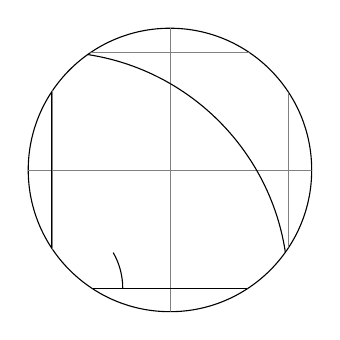
\begin{tikzpicture}[scale=3]
  \clip[draw] (0.5,0.5) circle (.6cm);
  \draw[step=.5cm,gray,very thin] (-1.4,-1.4) grid (1.4,1.4);
  \draw (-1.5,0) -- (1.5,0);
  \draw (0,-1.5) -- (0,1.5);
  \draw (0,0) circle [radius=1cm];
  \draw (3mm,0mm) arc [start angle=0, end angle=30, radius=3mm];
\end{tikzpicture}
\end{codeexample}


% \subsection{Parabola and Sine Path Construction}
\subsection{抛物线和正弦线路径构造}

% Although Karl does not need them for his picture, he is pleased to learn that there are |parabola| and |sin| and |cos| path operations for adding parabolas and sine and cosine curves to the current path. For the |parabola| operation, the current point will lie on the parabola as well as the point given after the parabola operation. Consider the following example:

虽然卡尔在他的图中不需要它们,但是他很高兴地知道有 |parabola| 和 |sin| 以及 |cos| 路径操作,可以在当前路径上添加抛物线和正弦和余弦曲线。对于 |parabola| 操作,当前点将位于抛物线上,以及在抛物线操作后给定的点。考虑下面的例子:

%
\begin{codeexample}[]
\tikz \draw (0,0) rectangle (1,1)  (0,0) parabola (1,1);
\end{codeexample}

% It is also possible to place the bend somewhere else:

也可以将拐弯放置在其他位置:

%
\begin{codeexample}[]
\tikz \draw[x=1pt,y=1pt] (0,0) parabola bend (4,16) (6,12);
\end{codeexample}

% The operations |sin| and |cos| add a sine or cosine curve in the interval $[0,\pi/2]$ such that the previous current point is at the start of the curve and the curve ends at the given end point. Here are two examples:

操作 |sin| 和 |cos| 在区间$[0,\pi/2]$中添加一条正弦或余弦曲线,前一个点在曲线的起点,曲线在给定的终点结束。这里有两个例子:

%
\begin{codeexample}[]
A sine \tikz \draw[x=1ex,y=1ex] (0,0) sin (1.57,1); curve.
\end{codeexample}

\begin{codeexample}[]
\tikz \draw[x=1.57ex,y=1ex] (0,0) sin (1,1) cos (2,0) sin (3,-1) cos (4,0)
                            (0,1) cos (1,0) sin (2,-1) cos (3,0) sin (4,1);
\end{codeexample}


% \subsection{Filling and Drawing}
\subsection{填充和绘图}

% Returning to the picture, Karl now wants the angle to be ``filled'' with a very light green. For this he uses |\fill| instead of |\draw|. Here is what Karl does:

回到这张图片,卡尔现在想用一个非常浅的绿色来“填充”这个角度。他使用 |\fill| 而不是 |\draw| 。卡尔是这样做的:

%
\begin{codeexample}[]
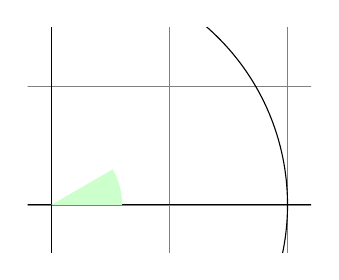
\begin{tikzpicture}[scale=3]
  \clip (-0.1,-0.2) rectangle (1.1,0.75);
  \draw[step=.5cm,gray,very thin] (-1.4,-1.4) grid (1.4,1.4);
  \draw (-1.5,0) -- (1.5,0);
  \draw (0,-1.5) -- (0,1.5);
  \draw (0,0) circle [radius=1cm];
  \fill[green!20!white] (0,0) -- (3mm,0mm)
    arc [start angle=0, end angle=30, radius=3mm] -- (0,0);
\end{tikzpicture}
\end{codeexample}

% The color |green!20!white| means 20\% green and 80\% white mixed together. Such color expression are possible since \tikzname\ uses Uwe Kern's |xcolor| package, see the documentation of that package for details on color expressions.

颜色 |green!20!white| 表示20\%的绿色和80\%的白色混合在一起。这样的颜色表达式是可能的,因为\tikzname\ 使用Uwe Kern编写的 |xcolor| 包,请参阅该包的文档以获得关于颜色表达式的详细信息。

% What would have happened, if Karl had not ``closed'' the path using |--(0,0)| at the end? In this case, the path is closed automatically, so this could have been omitted. Indeed, it would even have been better to write the following, instead:

如果卡尔没有使用 |--(0,0)|``闭合''路径在最后会发生什么?在本例中,路径会自动闭合,因此可以省略它。事实上,写以下代码甚至更好:

%
\begin{codeexample}[code only]
  \fill[green!20!white] (0,0) -- (3mm,0mm)
    arc [start angle=0, end angle=30, radius=3mm] -- cycle;
\end{codeexample}
%
%The |--cycle| causes the current path to be closed (actually the current part of the current path) by smoothly joining the first and last point. To appreciate the difference, consider the following example:

|--cycle| 通过平滑地连接第一个点和最后一个点,使当前路径闭合(事实上是当前路径的当前部分)。要了解差异,请考虑以下示例:

%
\begin{codeexample}[]
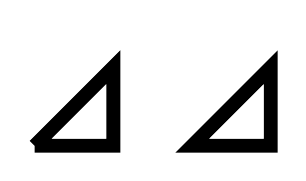
\begin{tikzpicture}[line width=5pt]
  \draw (0,0) -- (1,0) -- (1,1) -- (0,0);
  \draw (2,0) -- (3,0) -- (3,1) -- cycle;
  \useasboundingbox (0,1.5); % make bounding box higher
\end{tikzpicture}
\end{codeexample}

% You can also fill and draw a path at the same time using the |\filldraw| command. This will first draw the path, then fill it. This may not seem too useful, but you can specify different colors to be used for filling and for stroking. These are specified as optional arguments like this:

您还可以同时使用 |\filldraw| 命令来填充和绘制路径。这将首先绘制路径,然后填充它。这看起来可能不是很有用,但是你可以指定不同的颜色来填充和描边。这些被指定为可选参数,像这样:

%
\begin{codeexample}[]
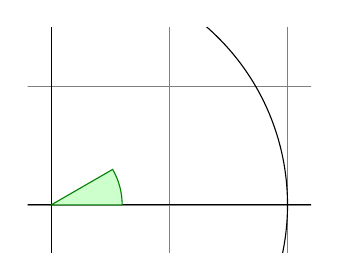
\begin{tikzpicture}[scale=3]
  \clip (-0.1,-0.2) rectangle (1.1,0.75);
  \draw[step=.5cm,gray,very thin] (-1.4,-1.4) grid (1.4,1.4);
  \draw (-1.5,0) -- (1.5,0);
  \draw (0,-1.5) -- (0,1.5);
  \draw (0,0) circle [radius=1cm];
  \filldraw[fill=green!20!white, draw=green!50!black] (0,0) -- (3mm,0mm)
    arc [start angle=0, end angle=30, radius=3mm] -- cycle;
\end{tikzpicture}
\end{codeexample}


% \subsection{Shading}
\subsection{阴影}

% Karl briefly considers the possibility of making the angle ``more fancy'' by \emph{shading} it. Instead of filling the area with a uniform color, a smooth transition between different colors is used. For this, |\shade| and |\shadedraw|, for shading and drawing at the same time, can be used:

卡尔简要地考虑了通过“阴影”使角度“更精致”的可能性。不使用统一的颜色填充区域,而是使用不同颜色之间的平滑过渡。为此,|\shade| 和 |\shadedraw| 可以同时添加阴影和进行绘图操作。

%
\begin{codeexample}[]
  \tikz \shade (0,0) rectangle (2,1)  (3,0.5) circle (.5cm);
\end{codeexample}
%
% The default shading is a smooth transition from gray to white. To specify different colors, you can use options:

默认的阴影是从灰色到白色的平滑过渡。要指定不同的颜色,您可以使用选项:

%
\begin{codeexample}[]

\begin{tikzpicture}[rounded corners,ultra thick]
  \shade[top color=yellow,bottom color=black] (0,0) rectangle +(2,1);
  \shade[left color=yellow,right color=black] (3,0) rectangle +(2,1);
  \shadedraw[inner color=yellow,outer color=black,draw=yellow] (6,0) rectangle +(2,1);
  \shade[ball color=green] (9,.5) circle (.5cm);
\end{tikzpicture}
\end{codeexample}

% For Karl, the following might be appropriate:

对于卡尔来说,以下代码可能是合适的:

%
\begin{codeexample}[]
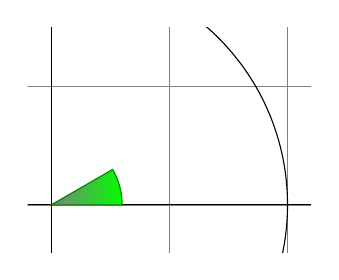
\begin{tikzpicture}[scale=3]
  \clip (-0.1,-0.2) rectangle (1.1,0.75);
  \draw[step=.5cm,gray,very thin] (-1.4,-1.4) grid (1.4,1.4);
  \draw (-1.5,0) -- (1.5,0);
  \draw (0,-1.5) -- (0,1.5);
  \draw (0,0) circle [radius=1cm];
  \shadedraw[left color=gray,right color=green, draw=green!50!black]
    (0,0) -- (3mm,0mm)
    arc [start angle=0, end angle=30, radius=3mm] -- cycle;
\end{tikzpicture}
\end{codeexample}

% However, he wisely decides that shadings usually only distract without adding anything to the picture.

然而,他明智地决定阴影通常只会分散注意力,而没有给图片添加任何东西。


%\subsection{Specifying Coordinates}
\subsection{指定坐标}

% Karl now wants to add the sine and cosine lines. He knows already that he can use the |color=| option to set the lines' colors. So, what is the best way to specify the coordinates?

卡尔现在想要加上正弦和余弦线。他已经知道可以使用 |color=| 选项来设置线条的颜色。那么,指定坐标的最好方法是什么?

% There are different ways of specifying coordinates. The easiest way is to say something like |(10pt,2cm)|. This means 10pt in $x$-direction and 2cm in $y$-directions. Alternatively, you can also leave out the units as in |(1,2)|, which means ``one times the current $x$-vector plus twice the current $y$-vector''. These vectors default to 1 cm in the $x$-direction and 1 cm in the $y$-direction, respectively.

有不同的方式来指定坐标。最简单的方法是像 |(10pt,2cm)| 这样。这意味着在$x$方向上的坐标为10pt,在$y$方向上的坐标为2cm。或者,您也可以省略单位 |(1,2)|,这意味着“当前$x$向量的1倍以及当前$y$向量的2倍”。向量默认在$x$方向上为1 cm,在$y$方向上为1 cm。

% In order to specify points in polar coordinates, use the notation |(30:1cm)|, which means 1 cm in direction 30 degree. This is obviously quite useful to ``get to the point $(\cos 30^\circ,\sin 30^\circ)$ on the circle''.

为了在极坐标中指定点,使用符号 |(30:1cm)|,意思是在30度方向上且极径为1 cm。这显然是非常有用的,以``得到圆上的点$(\cos 30^\circ,\sin 30^\circ)$''。

% You can add a single |+| sign in front of a coordinate or two of them as in |+(0cm,1cm)| or |++(2cm,0cm)|. Such coordinates are interpreted differently: The first form means ``1 cm upwards from the previous specified position'' and the second means ``2 cm to the right of the previous specified position, making this the new specified position''. For example, we can draw the sine line as follows:

您可以在坐标前添加一个或两个 |+| 符号,如 |+(0cm,1cm)| 或 |++(2cm,0cm)|。这些坐标的解释是不同的:第一种形式表示“上一指定位置上方1 cm”,第二种形式表示“上一指定位置右方2 cm,使其成为新的指定位置”。例如,我们可以画出正弦线如下:

%
\begin{codeexample}[]
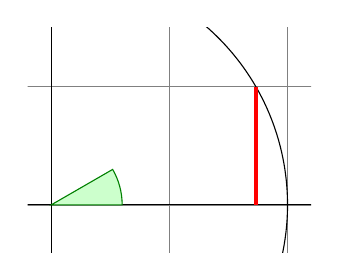
\begin{tikzpicture}[scale=3]
  \clip (-0.1,-0.2) rectangle (1.1,0.75);
  \draw[step=.5cm,gray,very thin] (-1.4,-1.4) grid (1.4,1.4);
  \draw (-1.5,0) -- (1.5,0);
  \draw (0,-1.5) -- (0,1.5);
  \draw (0,0) circle [radius=1cm];
  \filldraw[fill=green!20,draw=green!50!black] (0,0) -- (3mm,0mm)
      arc [start angle=0, end angle=30, radius=3mm] -- cycle;
  \draw[red,very thick] (30:1cm) -- +(0,-0.5);
\end{tikzpicture}
\end{codeexample}

% Karl used the fact $\sin 30^\circ = 1/2$. However, he very much doubts that his students know this, so it would be nice to have a way of specifying ``the point straight down from |(30:1cm)| that lies on the $x$-axis''. This is, indeed, possible using a special syntax: Karl can write \verb!(30:1cm |- 0,0)!. In general, the meaning of (\meta{p} \verb!|-! \meta{q}) is ``the intersection of a vertical line through $p$ and a horizontal line through $q$''.

卡尔使用了$\sin 30^\circ = 1/2$这个事实。然而,他很怀疑他的学生是否知道这一点,所以如果有一种方法来指定点从 |(30:1cm)| 径直向下绘制到在$x$轴上的点就好了。这确实是可能的,使用一种特殊的语法:Karl可以用 \verb!(30:1cm |- 0,0)!。一般来说,(\meta{p} \verb!|-! \meta{q})是“通过$p$的竖直线和通过$q$的水平线的交点”。

% Next, let us draw the cosine line. One way would be to say \verb!(30:1cm |- 0,0) -- (0,0)!. Another way is the following: we ``continue'' from where the sine ends:

接下来,我们来画余弦线。一种方法是 \verb!(30:1cm |- 0,0) -- (0,0)!。另一种方法是这样的:我们从正弦结束的地方``继续'':

%
\begin{codeexample}[]
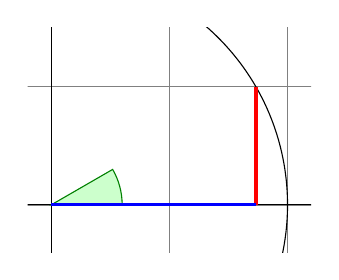
\begin{tikzpicture}[scale=3]
  \clip (-0.1,-0.2) rectangle (1.1,0.75);
  \draw[step=.5cm,gray,very thin] (-1.4,-1.4) grid (1.4,1.4);
  \draw (-1.5,0) -- (1.5,0);
  \draw (0,-1.5) -- (0,1.5);
  \draw (0,0) circle [radius=1cm];
  \filldraw[fill=green!20,draw=green!50!black] (0,0) -- (3mm,0mm)
      arc [start angle=0, end angle=30, radius=3mm] -- cycle;
  \draw[red,very thick]  (30:1cm) -- +(0,-0.5);
  \draw[blue,very thick] (30:1cm) ++(0,-0.5) -- (0,0);
\end{tikzpicture}
\end{codeexample}

% Note that there is no |--| between |(30:1cm)| and |++(0,-0.5)|. In detail, this path is interpreted as follows: ``First, the |(30:1cm)| tells me to move by pen to $(\cos 30^\circ,1/2)$. Next, there comes another coordinate specification, so I move my pen there without drawing anything. This new point is half a unit down from the last position, thus it is at $(\cos 30^\circ,0)$. Finally, I move the pen to the origin, but this time drawing something (because of the |--|).''

注意,在 |(30:1cm)| 和 |++(0,-0.5)| 之间不存在 |--|。具体来说,这个路径解释如下:``首先,|(30:1cm)| 告诉我将笔移动到$(\cos 30^\circ,1/2)$。接下来,指定了另一个坐标点,所以我移动我的笔,但不绘制任何东西。这个新点比上一个位置下降了半个单位,因此它在$(\cos 30 ^\circ,0)$。最后,我把笔移到原点,但这次画一些东西(因为用到了 |--|)。''

% To appreciate the difference between |+| and |++| consider the following example:

要理解 |+| 和 |++| 的区别,请考虑下面的例子:

%
\begin{codeexample}[]
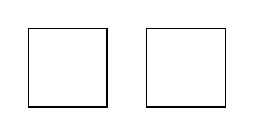
\begin{tikzpicture}
  \def\rectanglepath{-- ++(1cm,0cm)  -- ++(0cm,1cm)  -- ++(-1cm,0cm) -- cycle}
  \draw (0,0) \rectanglepath;
  \draw (1.5,0) \rectanglepath;
\end{tikzpicture}
\end{codeexample}

% By comparison, when using a single |+|, the coordinates are different:

通过比较,当使用单个 |+| 号时,坐标是不同的:

%
\begin{codeexample}[]
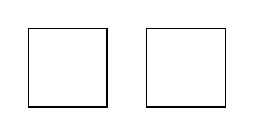
\begin{tikzpicture}
  \def\rectanglepath{-- +(1cm,0cm)  -- +(1cm,1cm)  -- +(0cm,1cm) -- cycle}
  \draw (0,0) \rectanglepath;
  \draw (1.5,0) \rectanglepath;
\end{tikzpicture}
\end{codeexample}


% Naturally, all of this could have been written more clearly and more economically like this (either with a single or a double |+|):

当然,所有这些都可以写成更清晰更经济的形式(一个或两个 |+| 号):


%
\begin{codeexample}[]
\tikz \draw (0,0) rectangle +(1,1)  (1.5,0) rectangle +(1,1);
\end{codeexample}


% \subsection{Intersecting Paths}
\subsection{相交路径}

% Karl is left with the line for $\tan \alpha$, which seems difficult to specify using transformations and polar coordinates. The first -- and easiest -- thing he can do is so simply use the coordinate |(1,{tan(30)})| since \tikzname's math engine knows how to compute things like |tan(30)|. Note the added braces since, otherwise, \tikzname's parser would think that the first closing parenthesis ends the coordinate (in general, you need to add braces around components of coordinates when these components contain parentheses).

留给卡尔的是$\tan\alpha$这一条线,这似乎很难使用变换和极坐标来指定。他能做的第一个也是最简单的事情就是使用坐标 |(1,{tan(30)})|,因为\tikzname 的数学引擎知道如何计算像 |tan(30)| 这样的东西。注意添加的大括号,否则\tikzname 的解析器会认为第一个右括号结束了坐标(通常,当坐标中包含括号时,需要坐标周围添加大括号)。

% Karl can, however, also use a more elaborate, but also more ``geometric'' way of computing the length of the orange line: He can specify intersections of paths as coordinates. The line for $\tan \alpha$ starts at $(1,0)$ and goes upward to a point that is at the intersection of a line going ``up'' and a line going from the origin through |(30:1cm)|. Such computations are made available by the |intersections| library.

但是,卡尔还可以使用更复杂但更``几何''的方式来计算橙色线的长度:他可以将路径的交点指定为坐标。 $\tan\alpha$的线从$(1,0)$开始,并向上到达一个点,该点是这条“向上”的线和一条线从原点到 |(30:1cm)| 线的交点。 通过 |intersections| 库可以得到这样的计算。 

% What Karl must do is to create two ``invisible'' paths that intersect at the position of interest. Creating paths that are not otherwise seen can be done using the |\path| command without any options like |draw| or |fill|. Then, Karl can add the |name path| option to the path for later reference. Once the paths have been constructed, Karl can use the |name intersections| to assign names to the coordinate for later reference.

卡尔必须做的是创建两条“看不见的”路径,在感兴趣的位置相交。可以使用 |\path| 命令创建其他方式看不到的路径,而不需要任何如 |draw| 或 |fill| 的选项。然后,卡尔可以将 |name path| 选项添加到该路径以供以后参考。一旦构造好了路径,卡尔就可以使用 |name intersections| 为坐标分配名称,以供以后参考。

%
\begin{codeexample}[code only]
\path [name path=upward line] (1,0) -- (1,1);
\path [name path=sloped line] (0,0) -- (30:1.5cm); % a bit longer, so that there is an intersection

% (add `\usetikzlibrary{intersections}' after loading tikz in the preamble)
\draw [name intersections={of=upward line and sloped line, by=x}]
  [very thick,orange] (1,0) -- (x);
\end{codeexample}


% \subsection{Adding Arrow Tips}
\subsection{添加箭头}

% Karl now wants to add the little arrow tips at the end of the axes. He has noticed that in many plots, even in scientific journals, these arrow tips seem to be missing, presumably because the generating programs cannot produce them. Karl thinks arrow tips belong at the end of axes. His son agrees. His students do not care about arrow tips.

卡尔现在想在轴的末端添加小箭头。 他注意到在许多情节中,甚至在科学期刊中,这些箭头似乎都消失了,大概是因为生成程序无法生成它们。卡尔认为箭头尖端位于轴的末端。 他的儿子同意。 他的学生不关心箭头。

% It turns out that adding arrow tips is pretty easy: Karl adds the option |->| to the drawing commands for the axes:

事实证明,添加箭头非常容易:卡尔在绘图命令中为坐标轴添加 |->| 选项:

%
\begin{codeexample}[preamble={\usetikzlibrary{intersections}}]
\begin{tikzpicture}[scale=3]
  \clip (-0.1,-0.2) rectangle (1.1,1.51);
  \draw[step=.5cm,gray,very thin] (-1.4,-1.4) grid (1.4,1.4);
  \draw[->] (-1.5,0) -- (1.5,0);
  \draw[->] (0,-1.5) -- (0,1.5);
  \draw (0,0) circle [radius=1cm];
  \filldraw[fill=green!20,draw=green!50!black] (0,0) -- (3mm,0mm)
        arc [start angle=0, end angle=30, radius=3mm] -- cycle;
  \draw[red,very thick]    (30:1cm) -- +(0,-0.5);
  \draw[blue,very thick]   (30:1cm) ++(0,-0.5) -- (0,0);

  \path [name path=upward line] (1,0) -- (1,1);
  \path [name path=sloped line] (0,0) -- (30:1.5cm);
  \draw [name intersections={of=upward line and sloped line, by=x}]
        [very thick,orange] (1,0) -- (x);
\end{tikzpicture}
\end{codeexample}

% If Karl had used the option |<-| instead of |->|, arrow tips would have been put at the beginning of the path. The option |<->| puts arrow tips at both ends of the path.

如果卡尔使用选项 |<-| 而不是 |->|,箭头就会被放在路径的开始处。选项 |<->| 在路径的两端都放置箭头。

% There are certain restrictions to the kind of paths to which arrow tips can be added. As a rule of thumb, you can add arrow tips only to a single open ``line''. For example, you cannot add tips to, say, a rectangle or a circle. However, you can add arrow tips to curved paths and to paths that have several segments, as in the following examples:

对于可以添加箭头的路径类型,存在某些限制。 根据经验,您只能将箭头添加到一条开放的``线''中。 例如,您不能将箭头添加到例如矩形或圆形。 但是,您可以向弯曲路径和具有多个线段的路径添加箭头,如以下示例所示:

%
\begin{codeexample}[]
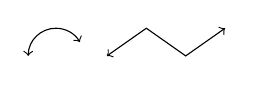
\begin{tikzpicture}
  \draw [<->] (0,0) arc [start angle=180, end angle=30, radius=10pt];
  \draw [<->] (1,0) -- (1.5cm,10pt) -- (2cm,0pt) -- (2.5cm,10pt);
\end{tikzpicture}
\end{codeexample}

% Karl has a more detailed look at the arrow that \tikzname\ puts at the end. It looks like this when he zooms it: \tikz[baseline] \draw[->,line width=1pt] (0pt,.5ex) -- ++(10pt,0pt);. The shape seems vaguely familiar and, indeed, this is exactly the end of \TeX's standard arrow used in something like $f\colon A \to B$.

卡尔详细观察发现\tikzname 把箭头放在了末端。当他放大时看起来像这样:\tikz[baseline] \draw[->,line width=1pt] (0pt,.5ex) -- ++(10pt,0pt);。形状似乎模糊不清,实际上,这恰好是\TeX 的标准箭头的末尾,用在$f\colon A \to B$之类的东西中。

% Karl likes the arrow, especially since it is not ``as thick'' as the arrows offered by many other packages. However, he expects that, sometimes, he might need to use some other kinds of arrow. To do so, Karl can say |>=|\meta{kind of end arrow tip}, where \meta{kind of end arrow tip} is a special arrow tip specification. For example, if Karl says |>=Stealth|, then he tells \tikzname\ that he would like  ``stealth-fighter-like'' arrow tips:

卡尔喜欢这个箭头,特别是因为它不是''像许多其他软件包提供的箭头''那样宽。然而,他希望,有时他可能需要使用一些其他种类的箭头。为此,卡尔可以用 |>=| \meta{末端箭头的类型},其中 \meta{末端箭头的类型} 是一个特殊的箭头规范。例如,如果卡尔用 |>=Stealth|,那么他告诉\tikzname\ 他想要“像隐形战斗机一样”的箭头:

\todosp{remaining instance of bug \#473}
%
\begin{codeexample}[preamble={\usetikzlibrary{arrows.meta}}]
\begin{tikzpicture}[>=Stealth]
  \draw [->] (0,0) arc [start angle=180, end angle=30, radius=10pt];
  \draw [<<-,very thick] (1,0) -- (1.5cm,10pt) -- (2cm,0pt) -- (2.5cm,10pt);
\end{tikzpicture}
\end{codeexample}

% Karl wonders whether such a military name for the arrow type is really necessary. He is not really mollified when his son tells him that Microsoft's PowerPoint uses the same name. He decides to have his students discuss this at some point.

卡尔想知道是否真的需要使用这种军事名称来表示箭头。 当儿子告诉他微软的PowerPoint也使用这样的名称时,他并没有真正感到高兴。 他决定让他的学生在某个时候对这个问题进行讨论。

% In addition to |Stealth| there are several other predefined kinds of arrow tips Karl can choose from, see Section~\ref{section-arrows}. Furthermore, he can define arrows types himself, if he needs new ones.

除了 |Stealth| 卡尔还可以选择其他几种预定义的箭头,请参见\ref {section-arrows}节。 此外,如果需要新的箭头类型,他可以自己定义箭头类型。


% \subsection{Scoping}
\subsection{分组}

% Karl saw already that there are numerous graphic options that affect how paths are rendered. Often, he would like to apply certain options to a whole set of graphic commands. For example, Karl might wish to draw three paths using a |thick| pen, but would like everything else to be drawn ``normally''.

卡尔已经看到,有许多图形选项会影响路径的渲染方式。 通常,他想将某些选项应用于整套图形命令。 例如,卡尔可能希望使用 |thick| 笔绘制三个路径。但希望其他所有东西都能``正常''绘制。

% If Karl wishes to set a certain graphic option for the whole picture, he can simply pass this option to the |\tikz| command or to the |{tikzpicture}| environment (Gerda would pass the options to |\tikzpicture| and Hans passes them to |\starttikzpicture|). However, if Karl wants to apply graphic options to a local group, he put these commands inside a |{scope}| environment (Gerda uses |\scope| and |\endscope|, Hans uses |\startscope| and |\stopscope|). This environment takes graphic options as an optional argument and these options apply to everything inside the scope, but not to anything outside. 

如果卡尔想为整个图片设置某个图形选项,他可以简单地将该选项传递给 |\tikz| 命令或 |{tikzpicture}| 环境(格达将把这些选项传递给 |\tikzpicture|, 汉森将它们传递给 |\starttikzpicture|)。但是,如果卡尔希望将图形选项应用到本地组,他可以将这些命令放在 |{scope}| 环境中(格达使用 |\scope| 和 |\endscope|, 汉森使用 |\startscope| 和 |\stopscope|)。该环境将图形选项作为可选参数,这些选项应用于范围内的所有内容,但不应用于范围外的任何内容。

% Here is an example:

这是一个案例:

%
\begin{codeexample}[]
\begin{tikzpicture}[ultra thick]
  \draw (0,0) -- (0,1);
  \begin{scope}[thin]
    \draw (1,0) -- (1,1);
    \draw (2,0) -- (2,1);
  \end{scope}
  \draw (3,0) -- (3,1);
\end{tikzpicture}
\end{codeexample}

% Scoping has another interesting effect: Any changes to the clipping area are local to the scope. Thus, if you say |\clip| somewhere inside a scope, the effect of the |\clip| command ends at the end of the scope. This is useful since there is no other way of ``enlarging'' the clipping area.

分组还有另一个有趣的作用:裁剪区域的任何更改都是该分组的局部更改。因此,如果您用 |\clip| 在某个分组内的某个地方,|\clip| 命令的效果将在分组的末尾结束。这是有用的,因为没有其他方式``扩大''剪切区域。

% Karl has also already seen that giving options to commands like |\draw| apply only to that command. It turns out that the situation is slightly more complex. First, options to a command like |\draw| are not really options to the command, but they are ``path options'' and can be given anywhere on the path. So, instead of |\draw[thin] (0,0) -- (1,0);| one can also write |\draw (0,0) [thin] -- (1,0);| or |\draw (0,0) -- (1,0) [thin];|; all of these have the same effect. This might seem strange since in the last case, it would appear that the |thin| should take effect only ``after'' the line from $(0,0)$ to $(1,0)$ has been drawn. However, most graphic options only apply to the whole path. Indeed, if you say both |thin| and |thick| on the same path, the last option given will ``win''.

卡尔也已经看到给像 |\draw| 这样的命令提供选项只适用于该命令。事实证明,情况要稍微复杂一些。首先,像 |\draw| 这样的命令的选项实际上并不是该命令的选项,但它们是“路径选项”,可以在路径的任何位置提供。因此,除了用 |\draw[thin] (0,0) -- (1,0);| 还可以用 |\draw (0,0) [thin] -- (1,0);| 或 |\draw (0,0) -- (1,0) [thin];|;所有这些都会产生同样的效果。这看起来可能有些奇怪,因为在上一种情况下,看起来 |thin| 应该只在从$(0,0)$到$(1,0)$这一行的``之后''才生效。但是,大多数图形选项只适用于整个路径。事实上,如果你将 |thin| 和 |thick| 用在同一条路径上,给出的最后一个选项将会``赢得胜利''。

% When reading the above, Karl notices that only ``most'' graphic options apply to the whole path. Indeed, all transformation options do \emph{not} apply to the whole path, but only to ``everything following them on the path''. We will have a more detailed look at this in a moment. Nevertheless, all options given during a path construction apply only to this path.

阅读以上内容时,卡尔注意到只有``大多数''图形选项适用于整个路径。 确实,所有变换选项都\emph{不会}适用于整个路径,而仅适用于``路径上遵循它们的所有内容''。 稍后我们将对此进行更详细的介绍。 但是,在路径构建过程中给出的所有选项仅适用于该路径。

% \subsection{Transformations}
\subsection{坐标变换}

% When you specify a  coordinate like |(1cm,1cm)|, where is that coordinate placed on the page? To determine the position, \tikzname, \TeX, and \textsc{pdf} or PostScript all apply certain transformations to the given coordinate in order to determine the final position on the page.

当您指定 |(1cm,1cm)| 之类的坐标时,该坐标在页面上的什么位置? 为了确定位置,\tikzname\ , \TeX 和\textsc{pdf}或PostScript都会使用一种确定的坐标变换,以确定其在页面上的最终位置。

% \tikzname\ provides numerous options that allow you to transform coordinates in \tikzname's private coordinate system. For example, the |xshift| option allows you to shift all subsequent points by a certain amount:

\tikzname\ 提供了许多选项,允许您在\tikzname 的私有坐标系统中变换坐标。例如,|xshift| 选项允许您将所有后续点移动一定距离:

\begin{codeexample}[]
\tikz \draw (0,0) -- (0,0.5) [xshift=2pt] (0,0) -- (0,0.5);
\end{codeexample}

% It is important to note that you can change transformation ``in the middle of a path'', a feature that is not supported by \pdf\ or PostScript. The reason is that \tikzname\ keeps track of its own transformation matrix. 

需要注意的是,您可以在``路径的中间''坐标变换,\pdf\ 或PostScript不支持这一特性。原因是\tikzname\ 会持续跟踪自己的坐标变换矩阵。

% Here is a more complicated example:

这是一个更复杂的示例:

%
\begin{codeexample}[]

\begin{tikzpicture}[even odd rule,rounded corners=2pt,x=10pt,y=10pt]
  \filldraw[fill=yellow!80!black] (0,0)   rectangle (1,1)
        [xshift=5pt,yshift=5pt]   (0,0)   rectangle (1,1)
                    [rotate=30]   (-1,-1) rectangle (2,2);
\end{tikzpicture}
\end{codeexample}

% The most useful transformations are |xshift| and |yshift| for shifting, |shift| for shifting to a given point as in |shift={(1,0)}| or |shift={+(0,0)}| (the braces are necessary so that \TeX\ does not mistake the comma for separating options), |rotate| for rotating by a certain angle (there is also a |rotate around| for rotating around a given point), |scale| for scaling by a certain factor, |xscale| and |yscale| for scaling only in the $x$- or $y$-direction (|xscale=-1| is a flip), and |xslant| and |yslant| for slanting. If these transformation and those that I have not mentioned are not sufficient, the |cm| option allows you to apply an arbitrary transformation matrix. Karl's students, by the way, do not know what a transformation matrix is.

最有用的坐标变换是用于平移的 |xshift| 和 |yshift| 变换,|shift| 变换将指定图形平移\verb|shift={(1,0)}|或 \verb|shift={+(0,0)}|中给定的距离(大括号是必需的,以便\TeX\ 不会将逗号分隔为选项),|rotate| 变换将指定图形旋转指定的角度(还有一个 |rotate around| 用于绕给定点旋转),|xscale| 和 |yscale| 用于将指定图形在$x$或$y$方向上缩放指定的倍数,|xslant| 和 |yslant| 用于图形的倾斜。如果这些变换以及我没有提到的变换都不足够,那么 |cm| 选项允许您应用任意变换矩阵。 顺便说一下,卡尔的学生不知道什么是变换矩阵。


% \subsection{Repeating Things: For-Loops}
\subsection{重复工作:For循环}

% Karl's next aim is to add little ticks on the axes at positions $-1$, $-1/2$, $1/2$, and $1$. For this, it would be nice to use some kind of ``loop'', especially since he wishes to do the same thing at each of these positions. There are different packages for doing this. \LaTeX\ has its own internal command for this, |pstricks| comes along with the powerful |\multido| command. All of these can be used together with \tikzname, so if you are familiar with them, feel free to use them. \tikzname\ introduces yet another command, called |\foreach|, which I introduced since I could never remember the syntax of the other packages. |\foreach| is defined in the package |pgffor| and can be used independently of \tikzname, but \tikzname\ includes it automatically.

卡尔的下一个目标是在$-1$,$-1/2$,$1/2$和$1$的位置的坐标轴上添加小刻度。为此,最好使用某种‘循环’,特别是因为他希望在这些位置上做同样的事情。可以使用不同的包来完成这项工作。\LaTeX\ 对此有自己的内部命令,|pstricks| 带有强大的 |\multido| 命令。所有这些都可以与\tikzname 一起使用,所以如果您熟悉它们,可以随意使用它们。\tikzname\ 引入了另一个命令 |\foreach|,我引入这个命令是因为我永远记不住其他宏包的语法。|\foreach| 命令定义在宏包 |pgffor| 中,可以独立于\tikzname 使用,但\tikzname\ 会自动包含它。

% In its basic form, the |\foreach| command is easy to use:

|\foreach| 命令的基本形式很容易使用:

%
\begin{codeexample}[]
\foreach \x in {1,2,3} {$x =\x$, }
\end{codeexample}

% The general syntax is |\foreach| \meta{variable}| in {|\meta{list of values}|} |\meta{commands}. Inside the \meta{commands}, the \meta{variable} will be assigned to the different values. If the \meta{commands} do not start with a brace, everything up to the next semicolon is used as \meta{commands}.

一般语法是 |\foreach| \meta{变量}| in {|\meta{值清单}|} |\meta{命令}。在\meta{命令} 内部,\meta{变量} 将分配给不同的值。如果 \meta{命令} 不是以大括号开头,则直到下一个分号的所有内容都将用作 \meta{命令}。

% For Karl and the ticks on the axes, he could use the following code:

对于卡尔,他可以使用以下代码绘制坐标轴上的刻度:

%
\begin{codeexample}[]
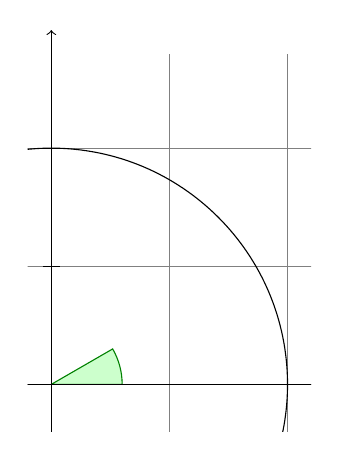
\begin{tikzpicture}[scale=3]
  \clip (-0.1,-0.2) rectangle (1.1,1.51);
  \draw[step=.5cm,gray,very thin] (-1.4,-1.4) grid (1.4,1.4);
  \filldraw[fill=green!20,draw=green!50!black] (0,0) -- (3mm,0mm)
      arc [start angle=0, end angle=30, radius=3mm] -- cycle;
  \draw[->] (-1.5,0) -- (1.5,0);
  \draw[->] (0,-1.5) -- (0,1.5);
  \draw (0,0) circle [radius=1cm];

  \foreach \x in {-1cm,-0.5cm,1cm}
    \draw (\x,-1pt) -- (\x,1pt);
  \foreach \y in {-1cm,-0.5cm,0.5cm,1cm}
    \draw (-1pt,\y) -- (1pt,\y);
\end{tikzpicture}
\end{codeexample}

% As a matter of fact, there are many different ways of creating the ticks. For example, Karl could have put the |\draw ...;| inside curly braces. He could also have used, say,

实际上,创建刻度线有很多不同的方法。 例如,卡尔可以将 |\draw ...;| 放在大括号内。 他还可以用,比如说,这样

%
\begin{codeexample}[code only]
\foreach \x in {-1,-0.5,1}
  \draw[xshift=\x cm] (0pt,-1pt) -- (0pt,1pt);
\end{codeexample}

% Karl is curious what would happen in a more complicated situation where there are, say, 20 ticks. It seems bothersome to explicitly mention all these numbers in the set for |\foreach|. Indeed, it is possible to use |...| inside the |\foreach| statement to iterate over a large number of values (which must, however, be dimensionless real numbers) as in the following example:

卡尔很好奇在更复杂的情况下会发生什么,比如说,20个刻度。为每个 |\foreach| 明确地提到集合中的所有数字似乎很麻烦。事实上,可以在 |\foreach| 声明中使用 |...| 产生大量迭代值(但是,它必须是无量纲的实数),如以下示例所示:

%
\begin{codeexample}[]
\tikz \foreach \x in {1,...,10}
        \draw (\x,0) circle (0.4cm);
\end{codeexample}

% If you provide \emph{two} numbers before the |...|, the |\foreach| statement will use their difference for the stepping:

如果在 |...| 之前提供\emph{2个}数字,则 |\foreach| 语句根据它们的差值进行步进:

%
\begin{codeexample}[]
\tikz \foreach \x in {-1,-0.5,...,1}
       \draw (\x cm,-1pt) -- (\x cm,1pt);
\end{codeexample}

% We can also nest loops to create interesting effects:

我们还可以使用嵌套循环以产生有趣的效果:

%
\begin{codeexample}[]
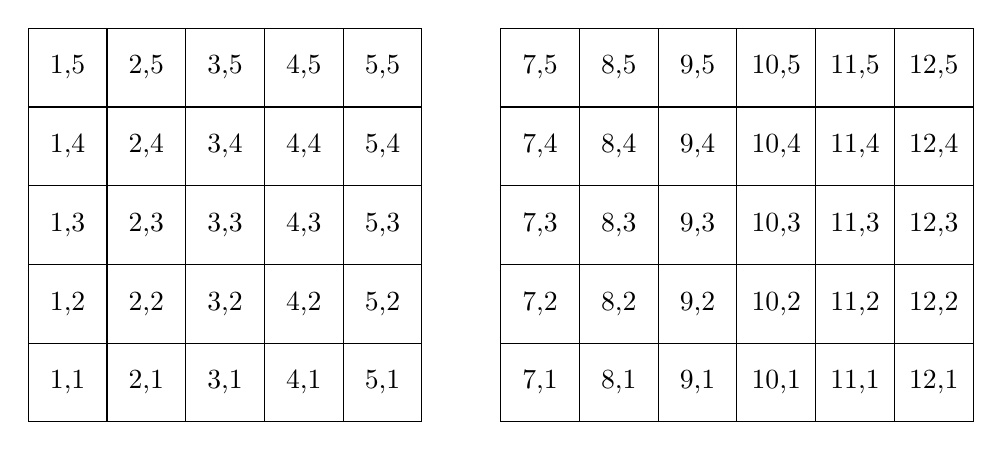
\begin{tikzpicture}
  \foreach \x in {1,2,...,5,7,8,...,12}
    \foreach \y in {1,...,5}
    {
      \draw (\x,\y) +(-.5,-.5) rectangle ++(.5,.5);
      \draw (\x,\y) node{\x,\y};
    }
\end{tikzpicture}
\end{codeexample}

% The |\foreach| statement can do even trickier stuff, but the above gives the idea.

|\foreach| 语句甚至可以做更棘手的事情,但是上面已经给出了这个想法。


% \subsection{Adding Text}
\subsection{添加文本}

% Karl is, by now, quite satisfied with the picture. However, the most important parts, namely the labels, are still missing!

到目前为止,卡尔对图片非常满意。 但是,最重要的部分,即文字标签,仍然缺失!

% \tikzname\ offers an easy-to-use and powerful system for adding text and, more generally, complex shapes to a picture at specific positions. The basic idea is the following: When \tikzname\ is constructing a path and encounters the keyword |node| in the middle of a path, it reads a \emph{node specification}. The keyword |node| is typically followed by some options and then some text between curly braces. This text is put inside a normal \TeX\ box (if the node specification directly follows a coordinate, which is usually the case, \tikzname\ is able to perform some magic so that it is even possible to use verbatim text inside the boxes) and then placed at the current position, that is, at the last specified position (possibly shifted a bit, according to the given options). However, all nodes are drawn only after the path has been completely drawn/filled/shaded/clipped/whatever.

\tikzname\ 提供了一个易于使用且功能强大的系统,用于在特定位置向图片添加文本和复杂形状。其基本思想如下:当\tikzname\ 构造路径并在路径中间遇到关键字 |node| 时,它读取\emph{节点详述}。关键字 |node| 后面通常跟着一些选项以及放在花括号之间的文本。这段文字放在普通的\TeX\ 盒子中(如果节点规范直接遵循坐标,并且通常就是这种情况,\tikzname\ 可以执行一些魔法般的操作,从而甚至可以在框中使用逐字记录文本),然后放在当前位置,即最后指定的位置(根据给定的选项,可能会移动一点)。但是,仅在完全绘制/填充/阴影/剪切或任何路径之后才绘制所有节点。

%
\begin{codeexample}[]
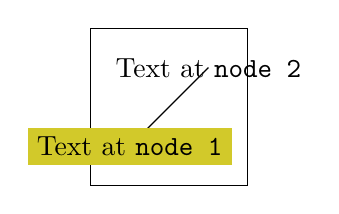
\begin{tikzpicture}
  \draw (0,0) rectangle (2,2);
  \draw (0.5,0.5) node [fill=yellow!80!black]
                       {Text at \verb!node 1!}
     -- (1.5,1.5) node {Text at \verb!node 2!};
\end{tikzpicture}
\end{codeexample}

% Obviously, Karl would not only like to place nodes \emph{on} the last specified position, but also to the left or the right of these positions. For this, every node object that you put in your picture is equipped with several \emph{anchors}. For example, the |north| anchor is in the middle at the upper end of the shape, the |south| anchor is at the bottom and the |north east| anchor is in the upper right corner. When you give the option |anchor=north|, the text will be placed such that this northern anchor will lie on the current position and the text is, thus, below the current position. Karl uses this to draw the ticks as follows:

显然,卡尔不仅希望将节点\emph{放置}在最后指定的位置,而是希望将其放置在这些位置的左侧或右侧。为此,你在图片中放置的每个节点对象都配备了多个\emph{锚点}。例如,|north| 锚点位于形状上端的中间,|south| 的锚点位于形状的底部,|north east| 的锚点位于形状的右上角。当提供选项 |anchor=north| 时,将放置文本,使得该北锚位于当前位置,因此该文本位于当前位置的下方。卡尔使用此方法绘制刻度线,如下所示:

%
\begin{codeexample}[]
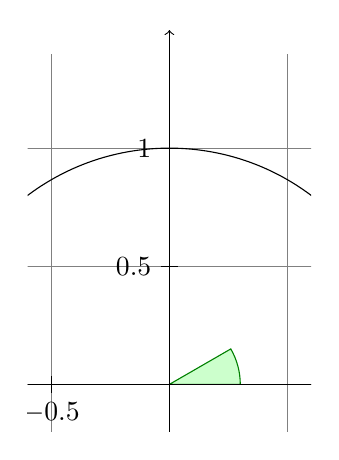
\begin{tikzpicture}[scale=3]
  \clip (-0.6,-0.2) rectangle (0.6,1.51);
  \draw[step=.5cm,help lines] (-1.4,-1.4) grid (1.4,1.4);
  \filldraw[fill=green!20,draw=green!50!black] (0,0) -- (3mm,0mm)
    arc [start angle=0, end angle=30, radius=3mm] -- cycle;
  \draw[->] (-1.5,0) -- (1.5,0);   \draw[->] (0,-1.5) -- (0,1.5);
  \draw (0,0) circle [radius=1cm];

  \foreach \x in {-1,-0.5,1}
    \draw (\x cm,1pt) -- (\x cm,-1pt) node[anchor=north] {$\x$};
  \foreach \y in {-1,-0.5,0.5,1}
    \draw (1pt,\y cm) -- (-1pt,\y cm) node[anchor=east] {$\y$};
\end{tikzpicture}
\end{codeexample}

% This is quite nice, already. Using these anchors, Karl can now add most of the other text elements. However, Karl thinks that, though ``correct'', it is quite counter-intuitive that in order to place something \emph{below} a given point, he has to use the \emph{north} anchor. For this reason, there is an option called |below|, which does the same as |anchor=north|. Similarly, |above right| does the same as |anchor=south west|. In addition, |below| takes an optional dimension argument. If given, the shape will additionally be shifted downwards by the given amount. So, |below=1pt| can be used to put a text label below some point and, additionally shift it  1pt downwards.

这已经很不错了。使用这些锚点,卡尔现在可以添加大多数的其他文本元素。然而,卡尔认为,虽然“正确”,但这是违反直觉的,为了把某些东西放在一个给定的点下面,他必须使用\emph{north}锚点。因此,有一个 |below| 的选项,它的作用与 |anchor=north| 相同。类似地,|above right| 与 |anchor=south wes| 的作用相同。另外,|below| 选项有一个可选的尺寸参数。如果给定,该形状将额外向下移动给定的数量。因此,|bellow=1pt| 可以用来把一个文本标签放在某个点下面,另外,将它向下移动1pt。

% Karl is not quite satisfied with the ticks. He would like to have $1/2$ or $\frac{1}{2}$ shown instead of $0.5$, partly to show off the nice capabilities of \TeX\ and \tikzname, partly because for positions like $1/3$ or $\pi$ it is certainly very much preferable to have the ``mathematical'' tick there instead of just the ``numeric'' tick. His students, on the other hand, prefer $0.5$ over $1/2$ since they are not too fond of fractions in general.

卡尔对刻度不太满意。他希望显示$1/2$或$\frac{1}{2}$而不是$0.5$,部分原因是为了展示\TeX\ 和\tikzname 的出色功能,部分原因是对于$1/3$或$\pi$这样的刻度,在上面放置``数学''的刻度而不是仅``数字的''刻度当然是更加可取的。 另一方面,他的学生更喜欢$0.5$而不是$1/2$,因为他们一般不太喜欢分数。

% Karl now faces a problem: For the |\foreach| statement, the position |\x| should still be given as |0.5| since \tikzname\ will not know where |\frac{1}{2}| is supposed to be. On the other hand, the typeset text should really be  |\frac{1}{2}|. To solve this problem, |\foreach| offers a special syntax: Instead of having one variable |\x|, Karl can specify two (or even more) variables separated by a slash as in |\x / \xtext|. Then, the elements in the set over which |\foreach| iterates must also be of the form \meta{first}|/|\meta{second}. In each iteration, |\x| will be set to \meta{first} and |\xtext| will be set to \meta{second}. If no \meta{second} is given, the \meta{first} will be used again. So, here is the new code for the ticks:

卡尔现在面临一个问题:对于 |\foreach| 声明,位置 |\x| 仍应为 |0.5|,因为\tikzname\ 不知道应该是 |\frac{1}{2}|。但另一方面,排版文本实际上应该是 |\frac{1}{2}|。要解决此问题,|\foreach| 提供了一种特殊的语法:与其使用一个变量 |\x|,卡尔可以指定两个(或更多)用斜杠分隔的变量 |\x / \xtext|。然后,集合中的元素使用 |\foreach| 迭代也必须采用 \meta{first}|/|\meta{second} 的形式。在每次迭代中,|\x| 将设置为 \meta{first},|\xtext| 将设置为 \meta{second}。如果没有给出 \meta{second},将再次使用 \meta{first}。因此,这是刻度的新代码:

%
\begin{codeexample}[]
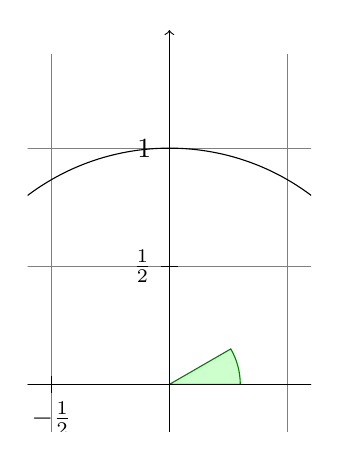
\begin{tikzpicture}[scale=3]
  \clip (-0.6,-0.2) rectangle (0.6,1.51);
  \draw[step=.5cm,help lines] (-1.4,-1.4) grid (1.4,1.4);
  \filldraw[fill=green!20,draw=green!50!black] (0,0) -- (3mm,0mm)
      arc [start angle=0, end angle=30, radius=3mm] -- cycle;
  \draw[->] (-1.5,0) -- (1.5,0); \draw[->] (0,-1.5) -- (0,1.5);
  \draw (0,0) circle [radius=1cm];

  \foreach \x/\xtext in {-1, -0.5/-\frac{1}{2}, 1}
    \draw (\x cm,1pt) -- (\x cm,-1pt) node[anchor=north] {$\xtext$};
  \foreach \y/\ytext in {-1, -0.5/-\frac{1}{2}, 0.5/\frac{1}{2}, 1}
    \draw (1pt,\y cm) -- (-1pt,\y cm) node[anchor=east] {$\ytext$};
\end{tikzpicture}
\end{codeexample}

% Karl is quite pleased with the result, but his son points out that this is still not perfectly satisfactory: The grid and the circle interfere with the numbers and decrease their legibility. Karl is not very concerned by this (his students do not even notice), but his son insists that there is an easy solution: Karl can add the |[fill=white]| option to fill out the background of the text shape with a white color.

卡尔对结果感到非常满意,但是他的儿子指出这仍然不能令人满意:网格和圆会干扰数字并降低其可读性。  卡尔对此并不十分担心(他的学生甚至没有注意到),但是他的儿子坚持认为有一个简单的解决方案:卡尔可以添加 \verb|[fill=white]| 选项,用白色填充文本形状的背景。

% The next thing Karl wants to do is to add the labels like $\sin \alpha$. For this, he would like to place a label ``in the middle of the line''. To do so, instead of specifying the label |node {$\sin\alpha$}|  directly after one of the endpoints of the line (which would place the label at that endpoint), Karl can give the label directly after the |--|, before the coordinate. By default, this places the label in the middle of the line, but the |pos=| options can be used to modify this. Also, options like |near start| and |near end| can be used to modify this position:

卡尔接下来要做的就是添加$\sin\alpha$之类的标签。为此,他想在线的中间放置一个标签。这样做,而不是指定标签 |node {$\sin\alpha$}| 直接在直线的一个端点之后(即将标签放置在端点处),卡尔可以在 |--| 之后,在坐标之前直接给出标签。缺省情况下,这会将标签放在行的中间,但是 |pos=| 选项可以用来修改它。另外,|near start| 和 |near end| 可以用来修改这个位置:
%
\begin{codeexample}[preamble={\usetikzlibrary{intersections}}]
\begin{tikzpicture}[scale=3]
  \clip (-2,-0.2) rectangle (2,0.8);
  \draw[step=.5cm,gray,very thin] (-1.4,-1.4) grid (1.4,1.4);
  \filldraw[fill=green!20,draw=green!50!black] (0,0) -- (3mm,0mm)
    arc [start angle=0, end angle=30, radius=3mm] -- cycle;
  \draw[->] (-1.5,0) -- (1.5,0) coordinate (x axis);
  \draw[->] (0,-1.5) -- (0,1.5) coordinate (y axis);
  \draw (0,0) circle [radius=1cm];

  \draw[very thick,red]
    (30:1cm) -- node[left=1pt,fill=white] {$\sin \alpha$} (30:1cm |- x axis);
  \draw[very thick,blue]
    (30:1cm |- x axis) -- node[below=2pt,fill=white] {$\cos \alpha$} (0,0);
  \path [name path=upward line] (1,0) -- (1,1);
  \path [name path=sloped line] (0,0) -- (30:1.5cm);
  \draw [name intersections={of=upward line and sloped line, by=t}]
    [very thick,orange] (1,0) -- node [right=1pt,fill=white]
    {$\displaystyle \tan \alpha \color{black}=
      \frac{{\color{red}\sin \alpha}}{\color{blue}\cos \alpha}$} (t);

  \draw (0,0) -- (t);

  \foreach \x/\xtext in {-1, -0.5/-\frac{1}{2}, 1}
    \draw (\x cm,1pt) -- (\x cm,-1pt) node[anchor=north,fill=white] {$\xtext$};
  \foreach \y/\ytext in {-1, -0.5/-\frac{1}{2}, 0.5/\frac{1}{2}, 1}
    \draw (1pt,\y cm) -- (-1pt,\y cm) node[anchor=east,fill=white] {$\ytext$};
\end{tikzpicture}
\end{codeexample}

% You can also position labels on curves and, by adding the |sloped| option, have them rotated such that they match the line's slope. Here is an example:

您也可以在曲线上放置标签,并通过添加 |sloped| 选项,使其旋转以使其与直线的斜率匹配。 这是一个例子:

%

\begin{codeexample}[]
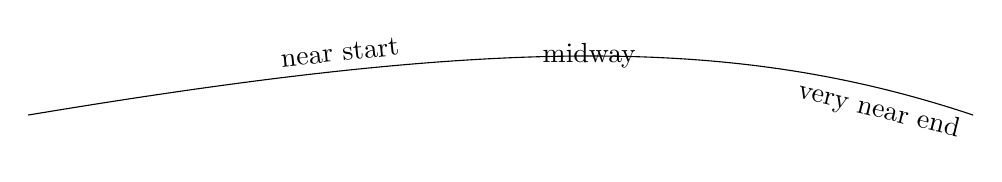
\begin{tikzpicture}
  \draw (0,0) .. controls (6,1) and (9,1) ..
    node[near start,sloped,above] {near start}
    node {midway}
    node[very near end,sloped,below] {very near end} (12,0);
\end{tikzpicture}
\end{codeexample}

% It remains to draw the explanatory text at the right of the picture. The main difficulty here lies in limiting the width of the text ``label'', which is quite long, so that line breaking is used. Fortunately, Karl can use the option |text width=6cm| to get the desired effect. So, here is the full code:

现在仍然需要在图片右侧绘制说明文字。 这里的主要困难在于限制文本``标签''的宽度,该宽度相当长,因为使用了换行符。幸运的是,卡尔可以使用选项 |text width=6cm|,以获得理想的效果。 因此,这是完整的代码:
%
\begin{codeexample}[code only]
\begin{tikzpicture}
  [scale=3,line cap=round,
  % Styles
  axes/.style=,
  important line/.style={very thick},
  information text/.style={rounded corners,fill=red!10,inner sep=1ex}]

  % Colors
  \colorlet{anglecolor}{green!50!black}
  \colorlet{sincolor}{red}
  \colorlet{tancolor}{orange!80!black}
  \colorlet{coscolor}{blue}

  % The graphic
  \draw[help lines,step=0.5cm] (-1.4,-1.4) grid (1.4,1.4);

  \draw (0,0) circle [radius=1cm];

  \begin{scope}[axes]
    \draw[->] (-1.5,0) -- (1.5,0) node[right] {$x$} coordinate(x axis);
    \draw[->] (0,-1.5) -- (0,1.5) node[above] {$y$} coordinate(y axis);

    \foreach \x/\xtext in {-1, -.5/-\frac{1}{2}, 1}
      \draw[xshift=\x cm] (0pt,1pt) -- (0pt,-1pt) node[below,fill=white] {$\xtext$};

    \foreach \y/\ytext in {-1, -.5/-\frac{1}{2}, .5/\frac{1}{2}, 1}
      \draw[yshift=\y cm] (1pt,0pt) -- (-1pt,0pt) node[left,fill=white] {$\ytext$};
  \end{scope}

  \filldraw[fill=green!20,draw=anglecolor] (0,0) -- (3mm,0pt)
    arc [start angle=0, end angle=30, radius=3mm];
  \draw (15:2mm) node[anglecolor] {$\alpha$};

  \draw[important line,sincolor]
    (30:1cm) -- node[left=1pt,fill=white] {$\sin \alpha$} (30:1cm |- x axis);

  \draw[important line,coscolor]
    (30:1cm |- x axis) -- node[below=2pt,fill=white] {$\cos \alpha$} (0,0);

  \path [name path=upward line] (1,0) -- (1,1);
  \path [name path=sloped line] (0,0) -- (30:1.5cm);
  \draw [name intersections={of=upward line and sloped line, by=t}]
    [very thick,orange] (1,0) -- node [right=1pt,fill=white]
    {$\displaystyle \tan \alpha \color{black}=
      \frac{{\color{red}\sin \alpha}}{\color{blue}\cos \alpha}$} (t);

  \draw (0,0) -- (t);

  \draw[xshift=1.85cm]
    node[right,text width=6cm,information text]
    {
      The {\color{anglecolor} angle $\alpha$} is $30^\circ$ in the
      example ($\pi/6$ in radians). The {\color{sincolor}sine of
        $\alpha$}, which is the height of the red line, is
      \[
      {\color{sincolor} \sin \alpha} = 1/2.
      \]
      By the Theorem of Pythagoras ...
    };
\end{tikzpicture}
\end{codeexample}


%\subsection{Pics: The Angle Revisited}
\subsection{Pics:再访Angle}

% Karl expects that the code of certain parts of the picture he created might be so useful that he might wish to reuse them in the future. A natural thing to do is to create \TeX\ macros that store the code he wishes to reuse. However, \tikzname\ offers another way that is integrated directly into its parser: pics!

卡尔希望他创建的图片某些部分的代码可能会非常有用,以至于他将来希望重用它们。 自然的做法是创建\TeX\ 宏来存储他希望重用的代码。 但是,\tikzname\ 提供了另一种直接集成到其解析器中的方式:图片!

% A ``pic'' is ``not quite a full picture'', hence the short name. The idea is that a pic is simply some code that you can add to a picture at different places using the |pic| command whose syntax is almost identical to the |node| command. The main difference is that instead of specifying some text in curly braces that should be shown, you specify the name of a predefined picture that should be shown.

``pic''是一种``不是很完整的图片'',因此我们使用简称。 这个想法是,图片只是一些代码,您可以使用 |pic| 命令添加到图片的不同位置, 它的语法几乎与 |node| 命令相同。 主要区别在于,您可以指定应该显示的预定义图片的名称,而不是在花括号中指定一些文本。

% Defining new pics is easy enough, see Section~\ref{section-pics}, but right now we just want to use one such predefined pic: the |angle| pic. As the name suggests, it is a small drawing of an angle consisting of a little wedge and an arc together with some text (Karl needs to load the |angles| library and the |quotes| for the following examples). What makes this pic useful is the fact that the size of the wedge will be computed automatically.

定义新的pics很容易,请参见\ref{section-pics}节,但是现在我们只想使用一个这样的预定义的pic:|angle| pic。顾名思义,这是一个由一张由一个楔形和一段弧以及一些文本组成的小图形(在以下示例中,卡尔需要加载 |angles| 和 |quotes| 库)。pic很有用的原因是,楔形的大小会被自动计算。

% The |angle| pic draws an angle between the two lines $BA$ and $BC$, where $A$, $B$, and $C$ are three coordinates. In our case, $B$ is the origin, $A$ is somewhere on the $x$-axis and $C$ is somewhere on a line at $30^\circ$.

|angle| pic在$BA$和$BC$两条线之间绘制一个角度,其中$A$、$B$和$C$是三个坐标。在我们的例子中,$B$是原点,$A$在$x$轴的某处,$C$在$30^\circ$这条线上的某处。
%
\begin{codeexample}[preamble={\usetikzlibrary{angles,quotes}}]
\begin{tikzpicture}[scale=3]
  \coordinate (A) at (1,0);
  \coordinate (B) at (0,0);
  \coordinate (C) at (30:1cm);

  \draw (A) -- (B) -- (C)
        pic [draw=green!50!black, fill=green!20, angle radius=9mm,
             "$\alpha$"] {angle = A--B--C};
\end{tikzpicture}
\end{codeexample}

% Let us see, what is happening here. First we have specified three \emph{coordinates} using the |\coordinate| command. It allows us to name a specific coordinate in the picture. Then comes something that starts as a normal |\draw|, but then comes the |pic| command. This command gets lots of options and, in curly braces, comes the most important point: We specify that we want to add an |angle| pic and this angle should be between the points we named |A|, |B|, and |C| (we could use other names). Note that the text that we want to be shown in the pic is specified in quotes inside the options of the |pic|, not inside the curly braces.

让我们来看看,这里发生了什么。首先,我们使用 |\coordinate| 命令指定了三个\emph{坐标点}。它允许我们在图片中对一个特定的坐标命名。然后是一个普通的 |\draw| 命令,然后是 |pic| 命令。这个命令有很多选项,在花括号中是最重要的一点:我们指定要添加一个 |angle| pic,这个角应该位于我们命名的 |A|、|B| 和 |C| 之间(我们也可以使用其他名称)。注意,我们希望在pic中显示的文本是在 |pic| 选项中的引号中指定的,而不是在花括号中。

% To learn more about pics, please see Section~\ref{section-pics}.

要了解有关pics的更多信息,请参见\ref{section-pics}节。

